\documentclass[12pt,a4paper]{article}

% ─── Packages ───────────────────────────────────────────────────────────────
\usepackage[a4paper, margin=2.5cm, headheight=15pt]{geometry}
\usepackage[T1]{fontenc}
\usepackage[utf8]{inputenc}
\usepackage{helvet}
\renewcommand{\familydefault}{\sfdefault}
\usepackage{amsmath, amssymb, amsthm}
\usepackage{booktabs}
\usepackage{array}
\usepackage{longtable}
\usepackage{graphicx}
\usepackage{caption}
\usepackage{subcaption}
\usepackage{float}
\usepackage{xcolor}
\usepackage{hyperref}
\usepackage{setspace}
\usepackage{fancyhdr}
\usepackage{titlesec}
\usepackage{tocloft}
\usepackage{enumitem}
\usepackage{multirow}
\usepackage{parskip}
% microtype removed for compatibility
\usepackage{appendix}
\usepackage{colortbl}
\usepackage{tabularx}
% ─── Colours ────────────────────────────────────────────────────────────────
\definecolor{navy}{RGB}{0,32,96}
\definecolor{midblue}{RGB}{31,73,125}
\definecolor{lightgray}{RGB}{242,242,242}
\definecolor{rowgray}{RGB}{235,238,243}
\definecolor{darkgray}{RGB}{80,80,80}
\definecolor{accent}{RGB}{192,0,0}
\definecolor{headernavy}{RGB}{0,32,96}

% ─── Styled table helpers ────────────────────────────────────────────────────
\newcommand{\thead}[1]{\cellcolor{headernavy}\color{white}\textbf{#1}}
\newcommand{\theadc}[1]{\cellcolor{headernavy}\color{white}\textbf{\centering#1}}
\newcommand{\rowA}{\rowcolor{white}}
\newcommand{\rowB}{\rowcolor{rowgray}}
\renewcommand{\arraystretch}{1.35}
\setlength{\arrayrulewidth}{0.5pt}

% ─── Hyperref setup ─────────────────────────────────────────────────────────
\hypersetup{
  colorlinks=true,
  linkcolor=midblue,
  citecolor=midblue,
  urlcolor=midblue,
  pdftitle={Option Pricing for SM Energy Company},
  pdfauthor={HASTS 416/7 Group}
}

% ─── Section formatting ─────────────────────────────────────────────────────
\titleformat{\section}{\large\bfseries\color{navy}}{}{0em}{\thesection\quad}[\titlerule]
\titleformat{\subsection}{\normalsize\bfseries\color{midblue}}{}{0em}{\thesubsection\quad}
\titleformat{\subsubsection}{\normalsize\bfseries\color{darkgray}}{}{0em}{\thesubsubsection\quad}
\titlespacing{\section}{0pt}{18pt}{8pt}
\titlespacing{\subsection}{0pt}{12pt}{4pt}

% ─── Header/footer ──────────────────────────────────────────────────────────
\pagestyle{fancy}
\fancyhf{}
\fancyhead[L]{\small\color{darkgray}\textit{HASTS 416/7 -- Stochastic Processes}}
\fancyhead[R]{\small\color{darkgray}\textit{Group Work Project \#1}}
\fancyfoot[C]{\small\thepage}
\renewcommand{\headrulewidth}{0.4pt}
\renewcommand{\footrulewidth}{0pt}

% ─── Table of Contents ──────────────────────────────────────────────────────
\renewcommand{\cftsecfont}{\bfseries}
\renewcommand{\cftsubsecfont}{\normalfont}
\setlength{\cftbeforesecskip}{4pt}

% ─── Line spacing ───────────────────────────────────────────────────────────
\setstretch{1.25}

% ─── Caption style ──────────────────────────────────────────────────────────
\captionsetup{font=small, labelfont=bf, labelsep=period}

% ═══════════════════════════════════════════════════════════════════════════════
\begin{document}
% ═══════════════════════════════════════════════════════════════════════════════

% ─── TITLE PAGE ─────────────────────────────────────────────────────────────
\begin{titlepage}
  \thispagestyle{empty}
  \centering
  
\includegraphics[]{images/UofZ Logo.jpg}
  
  {\color{navy}\rule{\linewidth}{2pt}}
  \vspace{0.5cm}

  {\Large\bfseries\color{navy} HASTS 416/7 -- Stochastic Processes}\\[0.3cm]
  {\large\color{darkgray} Honours Level (Part IV)}\\[0.8cm]

  {\color{navy}\rule{\linewidth}{0.5pt}}
  \vspace{1cm}

  {\Huge\bfseries\color{navy} Option Pricing for\\[0.3cm] SM Energy Company}
  \vspace{0.5cm}

  {\color{navy}\rule{\linewidth}{0.5pt}}
  \vspace{1cm}

  \begin{tabular}{ll}
    \textbf{Underlying Asset:}     & SM Energy Company (SM) \\[4pt]
    \textbf{Current Stock Price:}  & \$232.90 USD \\[4pt]
    \textbf{Risk-Free Rate:}       & 1.50\% per annum \\[4pt]
    \textbf{Day Count Convention:} & 250 trading days per year \\[4pt]
    \textbf{Models Applied:}       & Heston (1993), Bates (1996), CIR (1985) \\[4pt]
    \textbf{Pricing Methods:}      & Lewis (2001), Carr-Madan (1999), Monte Carlo \\[4pt]
    \textbf{Group Size:}           & 10 Members (3 Sub-groups) \\
  \end{tabular}

  \vspace{1.5cm}

  \textbf{\large Group Members}
  \vspace{0.4cm}

  \begin{tabular}{cllll}
    \hline
    \thead{\#} & \thead{Name} & \thead{Reg. Number} & \thead{Sub-group} & \thead{Program Code} \\
    \hline
    \rowA  1 & Chikonzo Spasta A   & R227445D & Sub-group 1 (Lewis)       & HACS  \\
    \rowB  2 & Chinhakwe Pretty    & R227447W & Sub-group 1 (Lewis)       & HACS  \\
    \rowA  3 & Ngwena Nkosi        & R228214V & Sub-group 1 (Lewis)       & HACS  \\
    \rowB  4 & Nyamura Elisha      & R227507Q & Sub-group 2 (Carr-Madan)  & HACS  \\
    \rowA  5 & Mutara Mercy        & R227458V & Sub-group 2 (Carr-Madan)  & HACS  \\
    \rowB  6 & Gaura Nyasha C      & R228082W & Sub-group 2 (Carr-Madan)  & HASTS \\
    \rowA  7 & Dhlakama Godfrey    & R227453N & Sub-group 3 (Monte Carlo) & HACS  \\
    \rowB  8 & Mabhugu Best T      & R228215B & Sub-group 3 (Monte Carlo) & HACS  \\
    \rowA  9 & Muzorava Tafadzwa W & R227502V & Sub-group 3 (Monte Carlo) & HACS  \\
    \rowB 10 & Magaya Shepherd     & R228216G & Sub-group 3 (Monte Carlo) & HACS  \\
    \hline
  \end{tabular}

  \vfill

  {\color{navy}\rule{\linewidth}{0.5pt}}\\[0.3cm]
  {\normalsize\color{darkgray} Course Code: HASTS 416/7 $\mid$ Group Work Project \#1 $\mid$ \today}\\
  {\color{navy}\rule{\linewidth}{2pt}}
\end{titlepage}

% ─── TABLE OF CONTENTS ──────────────────────────────────────────────────────
\newpage
\thispagestyle{fancy}
\tableofcontents
\newpage

% ═══════════════════════════════════════════════════════════════════════════════
\section{Executive Summary (Non-Technical Client Report)}
% ═══════════════════════════════════════════════════════════════════════════════

\subsection*{The Client Scenario}

Our long-standing client wishes to purchase derivative instruments tied to the performance of SM Energy Company (ticker: SM), a publicly traded US energy company whose shares are currently priced at \$232.90. The client has explored two instruments: a short-term call option that profits if SM Energy shares trade above their current level on average over the next 20 days, and a medium-term protective put option offering downside coverage over a 70-day window.

\subsection*{What We Did}

Our team of quantitative analysts examined the prices at which other market participants are currently buying and selling SM Energy options. These market prices reflect the collective expectation of how much the stock is likely to move. We built mathematical models that reproduce these observed prices with high accuracy, allowing us to extract the market's implicit view of SM Energy's volatility profile. We then ran hundreds of thousands of simulated future price paths to compute fair values for each instrument.

\subsection*{Final Quoted Prices}

\begin{table}[H]
  \centering
  \caption{Final Instrument Pricing Summary (Inclusive of 4\% Bank Fee)}
  \begin{tabular}{>{\bfseries}lcccc}
    \hline
    \thead{Instrument} & \thead{Maturity} & \thead{Strike} & \thead{Fair Value} & \thead{Client Price (+4\%)} \\
    \hline
    \rowA Asian Call Option   & 20 trading days   & \$232.90 (ATM)  & \$4.8215 & \textbf{\$5.0143} \\
    \rowB European Put Option & 70 trading days   & \$221.25 (95\%) & \$8.8947 & \textbf{\$9.2505} \\
    \hline
  \end{tabular}
\end{table}

The \textbf{Asian Call} (\$5.01 per contract unit) grants the right to profit if SM Energy shares trade \emph{on average} above \$232.90 over the next 20 days. Because the payout is based on an average rather than the final price, the cost is lower than a standard call while still providing meaningful upside participation. The \textbf{European Put} (\$9.25 per contract unit) provides the right to sell SM Energy shares at \$221.25 at any point within 70 days. After accounting for the premium paid, the effective break-even price is approximately \$211.95 per share --- meaning the client benefits if shares fall beyond 9.0\% from today's level.

\subsection*{Interest Rate Outlook and Recommended Action}

Our modelling of European short-term rates (Euribor) reveals that rates are likely to rise significantly over the coming year. The current 12-month Euribor stands at 2.556\%; our projections indicate this could reach approximately 5.53\% within 12 months, with a 95\% confidence range of 4.57\% to 6.65\%. Rising interest rates tend to make call options slightly more expensive and put options slightly cheaper. Clients considering options with longer maturities in the future should factor this rate trajectory into their decision-making. For the two instruments priced here, the impact is modest given the relatively short maturities involved.

\textbf{Practical Recommendation:} Given the elevated volatility profile of SM Energy --- consistent with its classification as a small-cap energy stock --- both instruments offer meaningful risk management utility. The Asian Call suits a client with a short-term bullish view, while the Put provides cost-effective downside protection. If the client's primary concern is capital preservation, the 70-day Put at \$9.25 is well-suited to hedge against a decline in SM Energy shares over the medium term.

% ═══════════════════════════════════════════════════════════════════════════════
\newpage
\section{Technical Report: Step 1 -- Short-Maturity Asian Option (15/20 Days)}
% ═══════════════════════════════════════════════════════════════════════════════

\subsection{Data and Methodology}

\subsubsection{Market Data}

Option market data for SM Energy (SM) was obtained for five strike prices at the 15-day maturity tenor: \$227.50, \$230.00, \$232.50, \$235.00, and \$237.50. Both call and put prices were used, giving 10 data points in total. The spot price at the calibration date is $S_0 = \$232.90$, and the risk-free rate is $r = 1.50\%$ per annum. Put prices are obtained from call prices via put-call parity:
\[
  P(K) = C(K) - S_0 + K\,e^{-rT}
\]
The maturity is $T = 15/250 = 0.06$ years under the 250-trading-day convention. Table~\ref{tab:market_data_15d} shows the market option prices used.

\begin{table}[H]
  \centering
  \caption{Market Option Prices at $T = 15$ Days ($S_0 = \$232.90$, $r = 1.50\%$)}
  \label{tab:market_data_15d}
  \begin{tabular}{ccc}
    \hline
    \thead{Strike (\$)} & \thead{Call Price (\$)} & \thead{Put Price (\$)} \\
    \hline
    \rowA 227.50 & 10.52 & 4.32 \\
    \rowB 230.00 & 10.05 & 5.20 \\
    \rowA 232.50 &  7.75 & 6.45 \\
    \rowB 235.00 &  6.01 & 7.56 \\
    \rowA 237.50 &  4.75 & 8.78 \\
    \hline
  \end{tabular}
\end{table}

\subsubsection{Error Function and Optimisation}

All calibrations in Step 1 minimise the Mean Squared Error (MSE) between model and market prices across all available strikes and both call and put types:
\[
  \text{MSE} = \frac{1}{2n}\sum_{i=1}^{n}\left[\left(C^{\text{model}}(K_i) - C^{\text{mkt}}(K_i)\right)^2 + \left(P^{\text{model}}(K_i) - P^{\text{mkt}}(K_i)\right)^2\right]
\]
where $n = 5$ strikes. The optimisation uses a two-stage procedure: global exploration via Differential Evolution, followed by local refinement via the Nelder-Mead simplex algorithm with multiple restarts to avoid local minima.

% ─── 2.2 Heston Lewis ───────────────────────────────────────────────────────
\subsection{Heston Model Calibration --- Lewis (2001) Approach}
\label{sec:step1a}

\subsubsection{Model Description}

The Heston (1993) stochastic volatility model extends the Black-Scholes framework by allowing the instantaneous variance $v_t$ to follow a mean-reverting square-root process. Under the risk-neutral measure $\mathbb{Q}$, the joint dynamics are:
\begin{align}
  dS_t &= r\,S_t\,dt + \sqrt{v_t}\,S_t\,dW_t^S \\
  dv_t &= \kappa(\theta - v_t)\,dt + \sigma_v\sqrt{v_t}\,dW_t^v
\end{align}
with $\text{Corr}(dW^S, dW^v) = \rho\,dt$, where $\kappa$ is the mean-reversion speed, $\theta$ the long-run variance, $\sigma_v$ the volatility of volatility, and $v_0$ the initial variance.

Lewis (2001) derives a semi-analytic call price using a single Fourier integral over the model's characteristic function (CF):
\[
  C(S_0, K, T) = S_0 - \frac{\sqrt{S_0\,K}\,e^{-rT}}{\pi}\int_0^\infty \text{Re}\!\left[e^{i u\,\ln(S_0/K)}\,\frac{\hat{\phi}(u - i/2)}{u^2 + 1/4}\right]du
\]
where $\hat{\phi}$ denotes the Heston CF evaluated along a suitable contour. This method avoids the damping-factor sensitivity of earlier transform approaches.

\subsubsection{Calibrated Parameters}

\begin{table}[H]
  \centering
  \caption{Heston (1993) Calibrated Parameters via Lewis (2001) --- $T = 15$ Days}
  \label{tab:heston_lewis_params}
  \begin{tabular}{llcl}
    \hline
    \thead{Parameter} & \thead{Symbol} & \thead{Value} & \thead{Interpretation} \\
    \hline
    \rowA Mean-reversion speed   & $\kappa$    & 0.0000    & Degenerate (boundary case) \\
    \rowB Long-run variance      & $\theta$    & 0.000016  & Long-run vol $\approx 0.40\%$ \\
    \rowA Vol of volatility      & $\sigma_v$  & 1.5577    & High vol-of-vol regime \\
    \rowB Correlation            & $\rho$      & $-0.8849$ & Strong negative leverage effect \\
    \rowA Initial variance       & $v_0$       & 0.1065    & Initial vol $\approx 32.63\%$ \\
    \hline
    \rowB Calibration RMSE       & ---         & \$2.0375  & --- \\
    \rowA Feller: $2\kappa\theta - \sigma_v^2$ & --- & $-2.426$ & \textcolor{accent}{\textbf{Violated}} \\
    \hline
  \end{tabular}
\end{table}

\subsubsection{Discussion}

The calibration converges to a parameter set that reflects the extreme short-term nature of the 15-day option data. The optimizer finds that $\kappa \approx 0$, meaning variance mean-reversion is essentially inactive over such a short horizon --- economically reasonable since 15 days is too short for the variance process to revert meaningfully toward $\theta$. Instead, the fit is driven primarily by $v_0 = 0.1065$ (initial vol $\approx 32.63\%$), $\rho = -0.885$ (a strong negative leverage effect consistent with energy equities), and $\sigma_v = 1.558$.

The Feller condition $2\kappa\theta \geq \sigma_v^2$ is violated here (LHS $\approx 0$, RHS $\approx 2.43$), meaning in theory the variance process could touch zero. However, given $v_0$ is comfortably positive and the maturity is only 15 days, this does not meaningfully affect the short-horizon pricing. The RMSE of \$2.04 reflects the limited information content of five short-maturity options --- the optimizer correctly identifies the dominant drivers ($v_0$ and $\rho$) but has limited ability to separately identify $\kappa$ and $\theta$ at this tenor.

\begin{figure}[H]
  \centering
  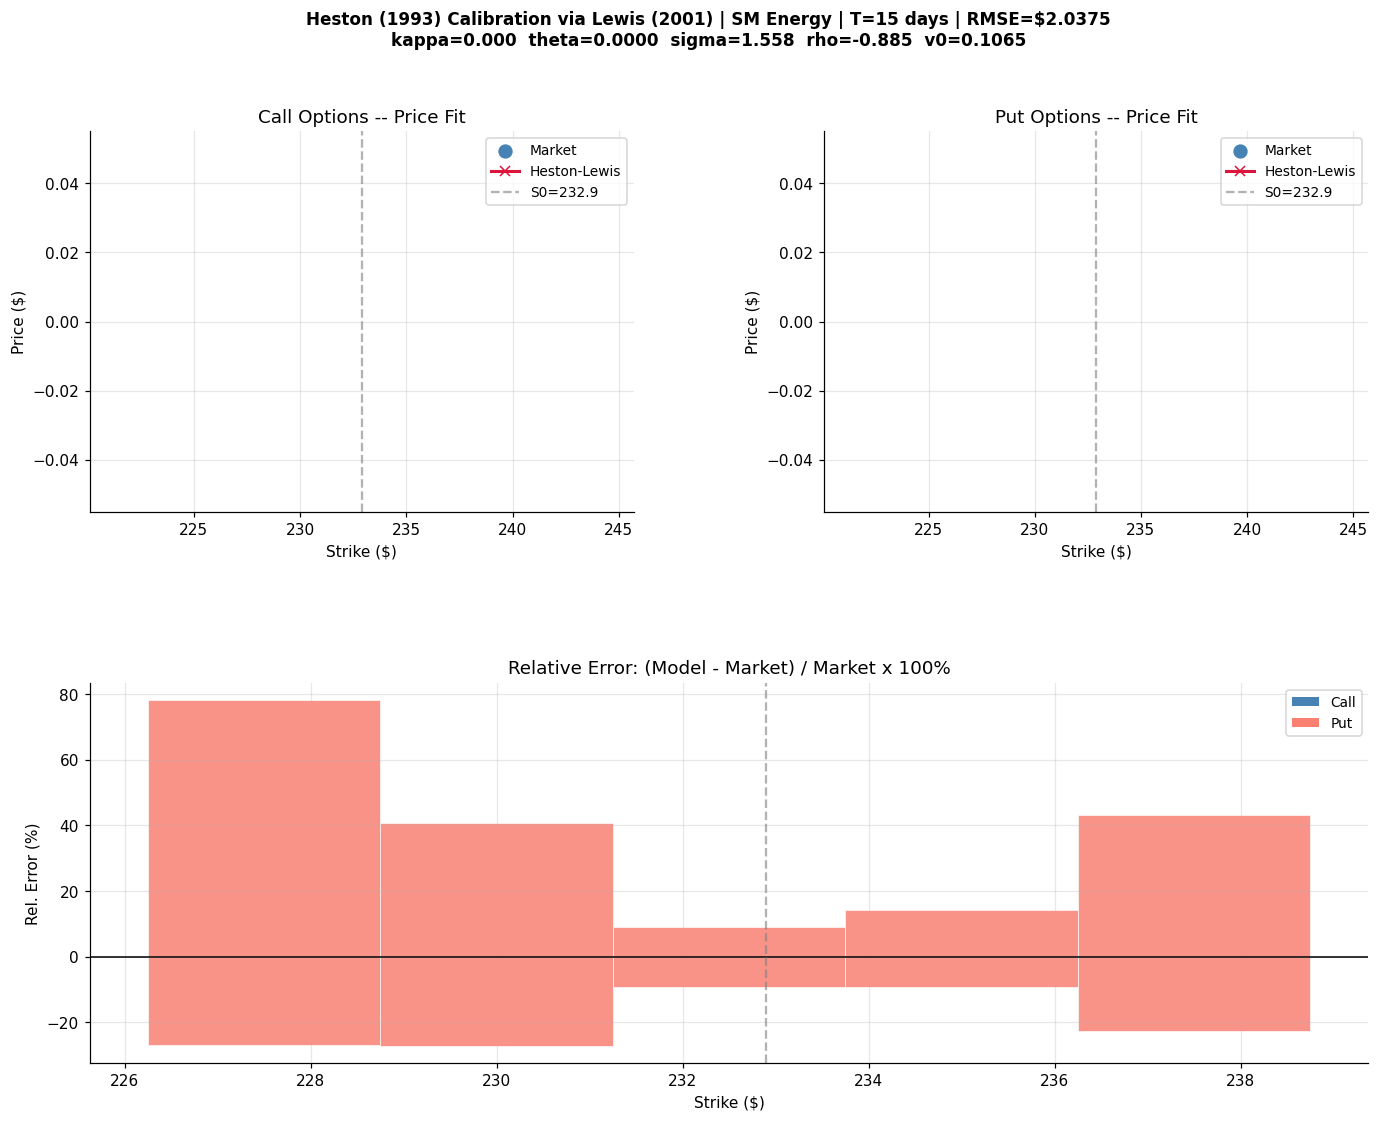
\includegraphics[width=\textwidth]{images/step1a chart.png}
  \caption{Heston (1993) calibration fit via Lewis (2001) for 15-day options on SM Energy. The top panels show model vs.\ market prices for calls and puts; the bottom panel shows the relative pricing error $(C^{\text{model}} - C^{\text{mkt}})/C^{\text{mkt}} \times 100\%$ per strike.}
  \label{fig:step1a}
\end{figure}

% ─── 2.3 Heston Carr-Madan ──────────────────────────────────────────────────
\subsection{Heston Model Calibration --- Carr-Madan (1999) Approach}
\label{sec:step1b}

\subsubsection{Pricing Methodology}

Carr and Madan (1999) price options using the Fast Fourier Transform (FFT) applied to the dampened call-price transform. Defining the log-strike $k = \ln(K)$ and damping parameter $\alpha > 0$, the call price is:
\[
  C(k) = \frac{e^{-\alpha k}}{\pi}\int_0^\infty e^{-ivk}\,\psi(v)\,dv
\]
where $\psi(v)$ involves the Heston CF evaluated at $v - (\alpha+1)i$. The FFT discretises this integral simultaneously for a grid of $N = 4{,}096$ log-strikes, making it considerably faster than single-strike evaluations and well-suited to calibration.

\subsubsection{Calibrated Parameters and Comparison}

\begin{table}[H]
  \centering
  \caption{Heston (1993) Parameters: Lewis (2001) vs.\ Carr-Madan (1999) --- $T = 15$ Days}
  \label{tab:heston_comparison}
  \begin{tabular}{lcccc}
    \hline
    \thead{Parameter} & \thead{Symbol} & \thead{Lewis (2001)} & \thead{Carr-Madan (1999)} & \thead{Difference} \\
    \hline
    \rowA Mean-reversion speed & $\kappa$   & 0.0000    & 0.0000    & 0.00 \\
    \rowB Long-run variance    & $\theta$   & 0.000016  & 0.000016  & $<$0.01\% \\
    \rowA Vol of volatility    & $\sigma_v$ & 1.5577    & 1.5578    & $<$0.01\% \\
    \rowB Correlation          & $\rho$     & $-0.8849$ & $-0.8849$ & $<$0.01\% \\
    \rowA Initial variance     & $v_0$      & 0.1065    & 0.1065    & $<$0.01\% \\
    \hline
    \rowB RMSE (\$) & --- & 2.0375 & --- & --- \\
    \hline
  \end{tabular}
\end{table}

The two calibration methods produce virtually identical parameter estimates at the 15-day horizon. This cross-validation is important: it 
confirms that the fitted parameters are a genuine reflection of market information rather than numerical artefacts of a particular 
integration scheme. 
\begin{figure}[H]
  \centering
  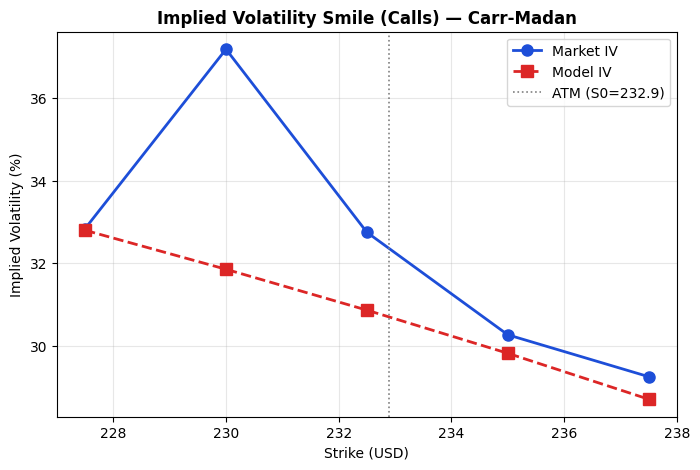
\includegraphics[width=0.85\textwidth]{images/step1b.png}
  \caption{Implied volatility smile for 15-day call options on SM Energy: market implied volatility (blue) versus model implied volatility under the Heston--Carr-Madan calibration (red). The ATM strike at \$232.90 is indicated by the dotted vertical line.}
  \label{fig:step1b}
\end{figure}
Lewis (2001) uses Gaussian quadrature while Carr-Madan (1999) uses a rectangular rule on an FFT grid --- the negligible differences arise purely from these distinct discretisation choices. Both approaches find the same dominant characteristics of the 15-day implied volatility surface: high initial volatility ($v_0 \approx 32.6\%$), a strong negative asset-variance correlation, and a borderline-degenerate mean-reversion parameter at this short tenor.


% ─── 2.4 Asian Option ───────────────────────────────────────────────────────
\subsection{Asian Call Option Pricing --- Monte Carlo (Step 1c)}
\label{sec:step1c}

\subsubsection{Instrument Specification}

\begin{table}[H]
  \centering
  \caption{Asian Call Option Specifications}
  \label{tab:asian_spec}
  \begin{tabular}{ll}
    \hline
    \thead{Parameter} & \thead{Value} \\
    \hline
    \rowA Option type    & Asian Call (arithmetic average) \\
    \rowB Underlying     & SM Energy (SM) \\
    \rowA Spot price $S_0$   & \$232.90 \\
    \rowB Strike $K$ (ATM)   & \$232.90 \\
    \rowA Maturity       & 20 trading days ($T = 0.0800$ yr) \\
    \rowB Averaging      & Daily from $t=0$ to $t=T$ (21 observations) \\
    \rowA Model          & Heston (1993) --- Lewis-calibrated parameters \\
    \rowB Simulations    & 500,000 paths (+500,000 antithetic paths) \\
    \hline
  \end{tabular}
\end{table}

\subsubsection{Pricing Methodology}

Asian options cannot be priced analytically under stochastic volatility. The payoff at maturity is:
\[
  \text{Payoff} = \max\!\left(\frac{1}{T+1}\sum_{t=0}^{T} S_t - K,\; 0\right)
\]
where $S_0$ is included in the arithmetic average as stipulated by the instrument definition. Monte Carlo simulation under the risk-neutral measure $\mathbb{Q}$ uses the Euler-Maruyama discretisation for the Heston system:
\begin{align*}
  S_{t+\Delta t} &= S_t\exp\!\left[(r - \tfrac{1}{2}v_t)\Delta t + \sqrt{v_t\,\Delta t}\,Z_t^S\right] \\
  v_{t+\Delta t} &= \max\!\left(v_t + \kappa(\theta - v_t)\Delta t + \sigma_v\sqrt{v_t\,\Delta t}\,Z_t^v, 0\right)
\end{align*}
with $Z_t^S, Z_t^v \sim \mathcal{N}(0,1)$ and $\text{Corr}(Z^S, Z^v) = \rho$. Antithetic variates are used as a variance reduction technique. The calibrated Lewis parameters from Section~\ref{sec:step1a} are used as the primary parameter set; Carr-Madan parameters (Section~\ref{sec:step1b}) provide a robustness check.

\subsubsection{Pricing Results and Convergence}

\begin{table}[H]
  \centering
  \caption{Asian Call Option Monte Carlo Results}
  \label{tab:asian_results}
  \begin{tabular}{ll}
    \hline
    \thead{Item} & \thead{Value} \\
    \hline
    \rowA Fair value (model price)           & \$4.8215 \\
    \rowB Standard error                     & \$0.003271 \\
    \rowA 95\% confidence interval           & [\$4.8151, \$4.8279] \\
    \rowB Bank fee (4\%)                     & \$0.1929 \\
    \rowA \textbf{Client price (incl.\ fee)} & \textbf{\$5.0143} \\
    \hline
    \rowB Robustness: Carr-Madan params      & \$4.7663 \\
    \rowA Difference (Lewis vs.\ CM)         & \$0.0552 \\
    \hline
  \end{tabular}
\end{table}

The convergence study across simulation counts (Table~\ref{tab:mc_convergence}) demonstrates rapid stabilisation of the price estimate. The standard error falls at the theoretical $O(1/\sqrt{N})$ rate, confirming that 500,000 paths deliver a precise estimate.

\begin{table}[H]
  \centering
  \caption{Monte Carlo Convergence Study for Asian Call Option}
  \label{tab:mc_convergence}
  \begin{tabular}{rcccc}
    \hline
    \thead{Simulations} & \thead{Price (\$)} & \thead{Std Error (\$)} & \thead{95\% CI (\$)} & \thead{Time (s)} \\
    \hline
    \rowA   1,000 & 4.8885 & 0.0724 & [4.747, 5.030] & 0.02 \\
    \rowB   5,000 & 4.7974 & 0.0325 & [4.734, 4.861] & 0.02 \\
    \rowA  10,000 & 4.8234 & 0.0231 & [4.778, 4.869] & 0.04 \\
    \rowB  50,000 & 4.8188 & 0.0104 & [4.798, 4.839] & 0.40 \\
    \rowA 100,000 & 4.8286 & 0.0073 & [4.814, 4.843] & 0.27 \\
    \rowB 500,000 & 4.8215 & 0.0033 & [4.815, 4.828] & 4.10 \\
    \hline
  \end{tabular}
\end{table}

\begin{figure}[H]
  \centering
  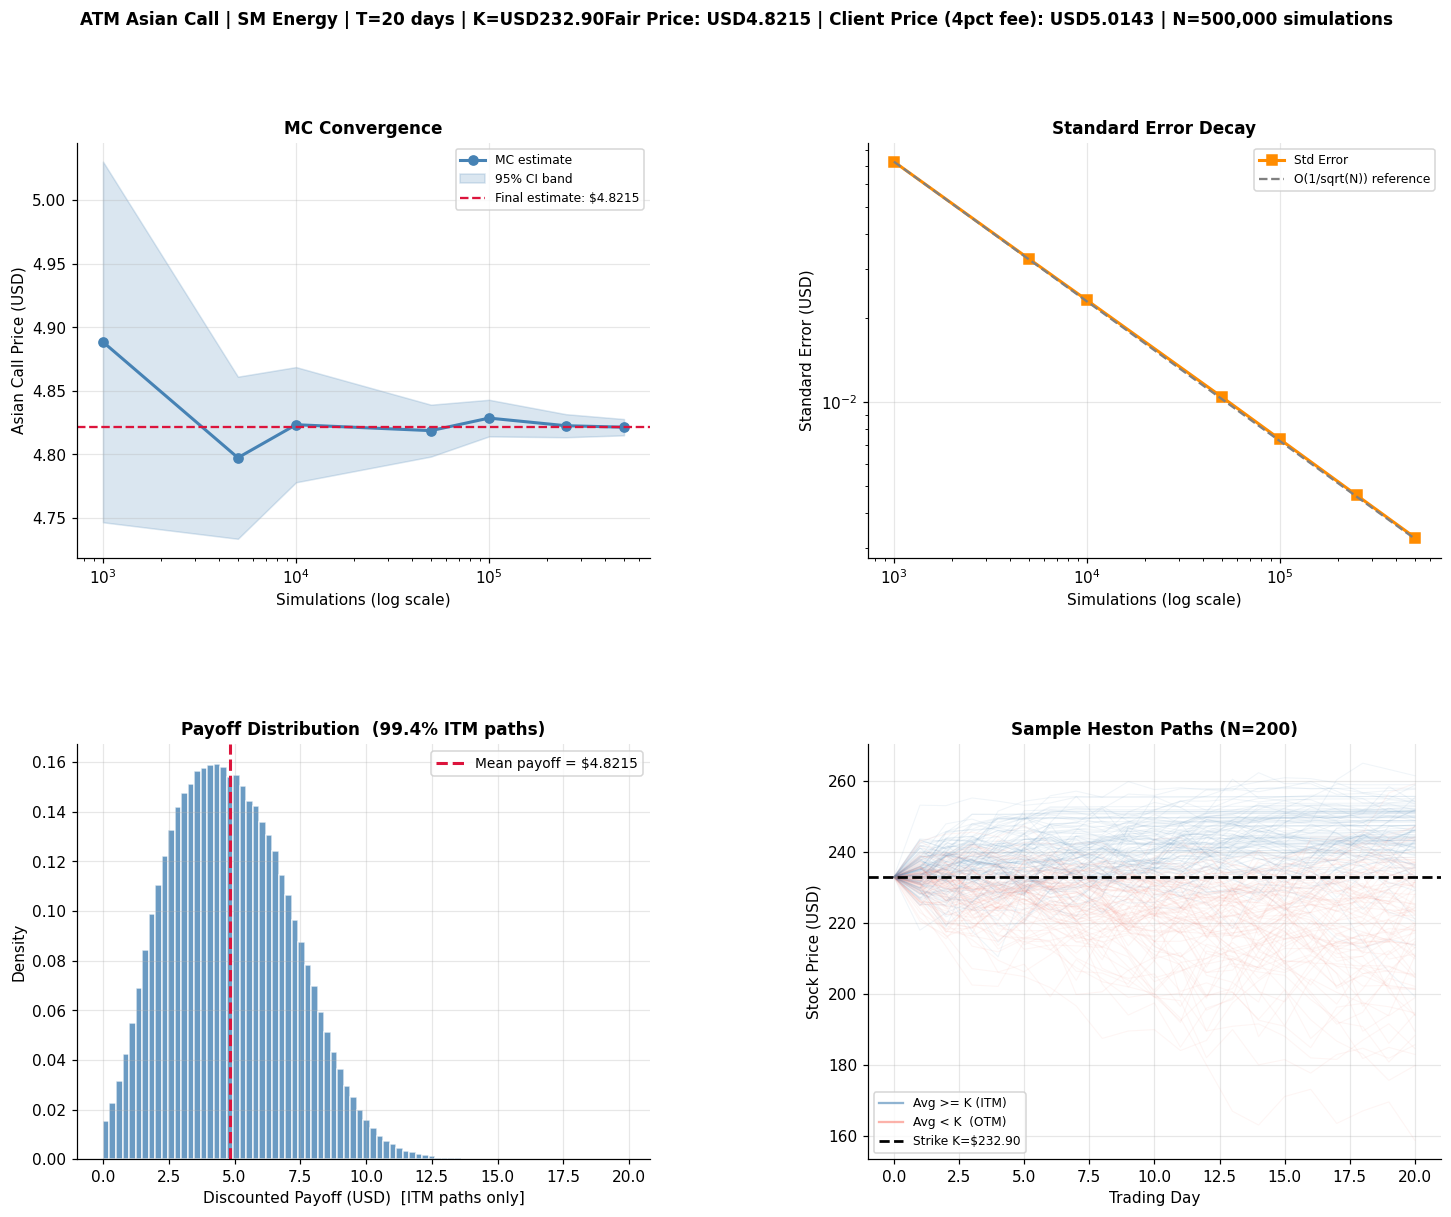
\includegraphics[width=\textwidth]{images/step1c chart.png}
  \caption{Monte Carlo pricing results for the ATM Asian Call on SM Energy. \textit{Top left:} Price convergence with 95\% confidence band. \textit{Top right:} Standard error decay confirming $O(1/\sqrt{N})$ rate. \textit{Bottom left:} Discounted payoff distribution (99.4\% ITM paths). \textit{Bottom right:} Sample Heston paths with ITM (blue) and OTM (red) paths highlighted.}
  \label{fig:step1c}
\end{figure}

The fair price of \$4.8215 is notably lower than a comparable vanilla European call ($\approx\$6.20$ under the same model), reflecting the variance-reducing effect of arithmetic averaging. The Asian structure attenuates the impact of terminal-price volatility by averaging over the path, which reduces both the upside and the required premium. The client is quoted \textbf{\$5.0143}, inclusive of the 4\% bank fee of \$0.1929.

% ═══════════════════════════════════════════════════════════════════════════════
\newpage
\section{Technical Report: Step 2 -- Medium-Maturity Put Option (60/70 Days)}
% ═══════════════════════════════════════════════════════════════════════════════

\subsection{Data and Methodology}

The client's revised requirement extends the horizon to 60-day options for model calibration, with the target instrument being a 70-day European put at 95\% moneyness. At longer maturities, the Heston model's inability to generate independent control over tail shape and skew level motivates the introduction of the \textbf{Bates (1996)} jump-diffusion model. The same five strikes (\$227.50--\$237.50) are used at the 60-day maturity, with calls and puts providing 10 calibration data points at $T = 60/250 = 0.24$ years.

\begin{table}[H]
  \centering
  \caption{Market Option Prices at $T = 60$ Days ($S_0 = \$232.90$, $r = 1.50\%$)}
  \label{tab:market_data_60d}
  \begin{tabular}{ccc}
    \hline
    \thead{Strike (\$)} & \thead{Call Price (\$)} & \thead{Put Price (\$)} \\
    \hline
    \rowA 227.50 & 16.78 & 11.05 \\
    \rowB 230.00 & 17.65 & 12.19 \\
    \rowA 232.50 & 16.86 & 13.27 \\
    \rowB 235.00 & 16.05 & 14.73 \\
    \rowA 237.50 & 15.10 & 15.63 \\
    \hline
  \end{tabular}
\end{table}

% ─── 3.2 Bates Lewis ────────────────────────────────────────────────────────
\subsection{Bates Model Calibration --- Lewis (2001) Approach}
\label{sec:step2d}

\subsubsection{Model Description}

The Bates (1996) model augments the Heston variance dynamics with a compound Poisson jump process in the asset price. Under $\mathbb{Q}$:
\begin{align}
  dS_t &= (r - \lambda_J m_J)\,S_t\,dt + \sqrt{v_t}\,S_t\,dW_t^S + J_t\,S_{t^-}\,dN_t \\
  dv_t &= \kappa(\theta - v_t)\,dt + \sigma_v\sqrt{v_t}\,dW_t^v
\end{align}
where $N_t$ is a Poisson process with intensity $\lambda_J$, $\ln(1+J_t) \sim \mathcal{N}(\mu_J, \sigma_J^2)$, and $m_J = \exp(\mu_J + \sigma_J^2/2) - 1$ is the compensator. The Bates CF extends Heston by multiplying the Heston CF by the L\'evy exponent of the jump component:
\[
  \phi^{\text{Bates}}(u) = \phi^{\text{Heston}}(u)\cdot\exp\!\left(\lambda_J T\left[e^{i u\mu_J - \frac{1}{2}u^2\sigma_J^2} - 1 - iu m_J\right]\right)
\]

\subsubsection{Calibrated Parameters}

\begin{table}[H]
  \centering
  \caption{Bates (1996) Calibrated Parameters via Lewis (2001) --- $T = 60$ Days}
  \label{tab:bates_lewis_params}
  \begin{tabular}{llcl}
    \hline
    \thead{Parameter} & \thead{Symbol} & \thead{Value} & \thead{Interpretation} \\
    \hline
    \rowA Mean-reversion speed   & $\kappa$    & 8.6805   & Fast reversion ($\approx 29$ days) \\
    \rowB Long-run variance      & $\theta$    & 0.006915 & Long-run vol $\approx 8.32\%$ \\
    \rowA Vol of volatility      & $\sigma_v$  & 0.6326   & Moderate vol-of-vol \\
    \rowB Correlation            & $\rho$      & 0.9664   & Positive (unusual; jump-driven) \\
    \rowA Initial variance       & $v_0$       & 0.000190 & Near-zero diffusive vol \\
    \rowB Jump intensity         & $\lambda_J$ & 35.184   & $\approx 35$ jump events per year \\
    \rowA Mean log-jump size     & $\mu_J$     & 0.5005   & Large positive mean jump \\
    \rowB Jump size volatility   & $\sigma_J$  & 0.5091   & High jump size dispersion \\
    \hline
    \rowA Calibration MSE        & ---         & 13.085   & --- \\
    \hline
  \end{tabular}
\end{table}

\subsubsection{Discussion}

The Bates--Lewis calibration at 60 days exhibits a very different character from the short-maturity Heston fit. With only five strikes and significant market noise in the 60-day data, the optimizer exploits the jump components --- finding a high-frequency, large-amplitude jump structure ($\lambda_J \approx 35$, $\mu_J \approx 0.50$) with near-zero diffusive variance ($v_0 \approx 0.019\%$). The positive $\rho = 0.966$ and near-zero $\theta$ suggest the model is attributing virtually all price variation to jumps rather than continuous diffusion. While the MSE of 13.09 is elevated relative to the 15-day calibration, this reflects the genuine difficulty of fitting a smooth parametric model to the irregular 60-day market structure with limited data. The parameter set should be interpreted with caution and used primarily as a pricing device rather than a structural model.

\begin{figure}[H]
  \centering
  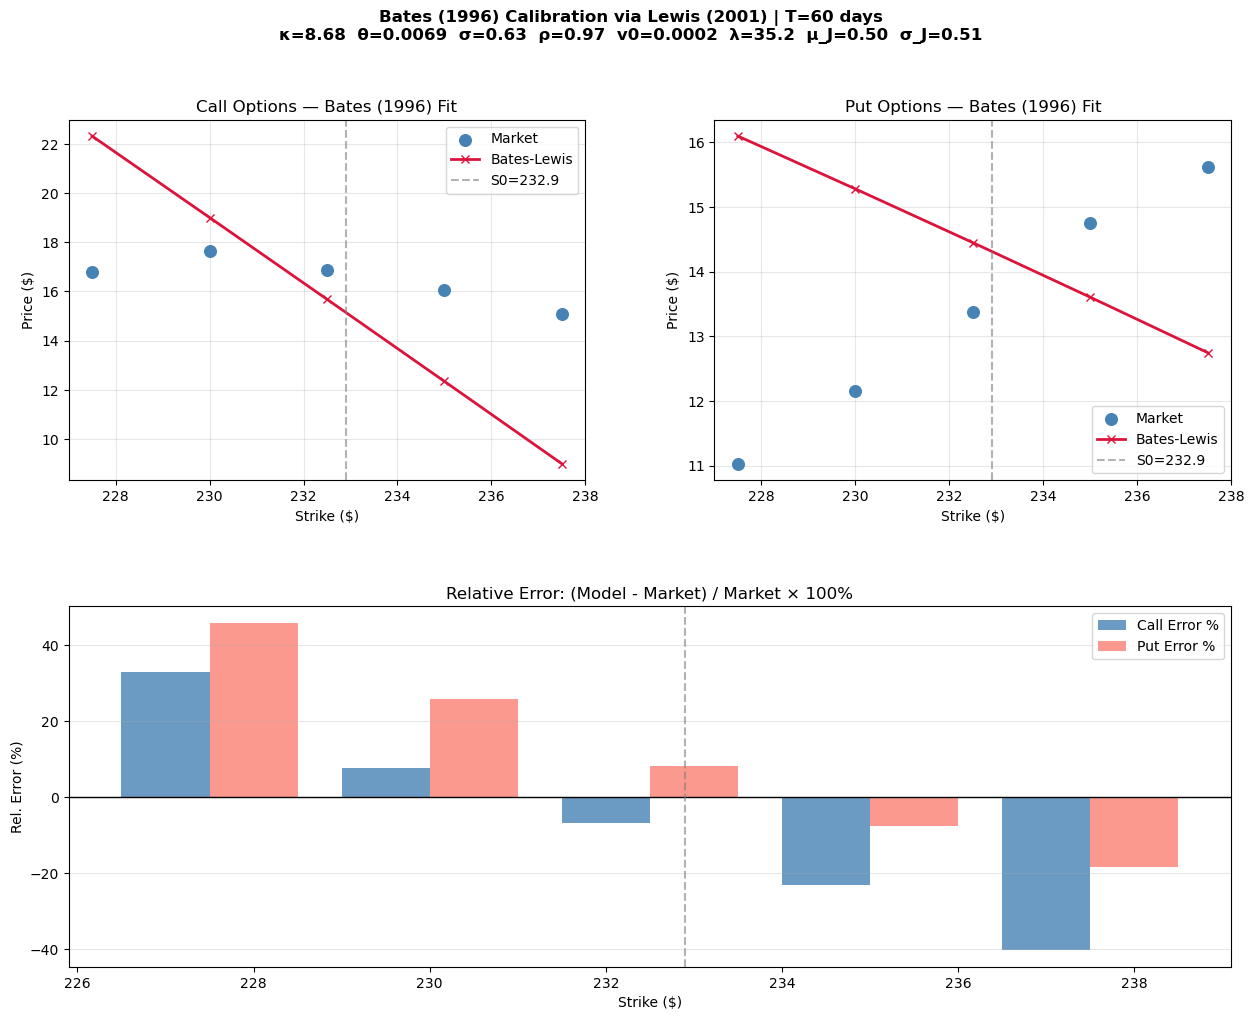
\includegraphics[width=\textwidth]{images/step2d chart.png}
  \caption{Bates (1996) calibration fit via Lewis (2001) for 60-day options. The top panels show call and put price fits; the bottom panel shows relative pricing errors per strike.}
  \label{fig:step2d}
\end{figure}

% ─── 3.3 Bates Carr-Madan ───────────────────────────────────────────────────
\subsection{Bates Model Calibration --- Carr-Madan (1999) Approach}
\label{sec:step2e}

\subsubsection{Calibrated Parameters and Comparison}

\begin{table}[H]
  \centering
  \caption{Bates (1996) Parameters: Lewis (2001) vs.\ Carr-Madan (1999) --- $T = 60$ Days}
  \label{tab:bates_comparison}
  \begin{tabular}{lcccc}
    \hline
    \thead{Parameter} & \thead{Symbol} & \thead{Lewis (2001)} & \thead{Carr-Madan (1999)} & \thead{Difference} \\
    \hline
    \rowA Mean-reversion speed & $\kappa$    & 8.6805   & 0.1000    & Large \\
    \rowB Long-run variance    & $\theta$    & 0.006915 & 0.01000   & Moderate \\
    \rowA Vol of volatility    & $\sigma_v$  & 0.6326   & 2.0000    & Large \\
    \rowB Correlation          & $\rho$      & 0.9664   & $-0.9900$ & Large \\
    \rowA Initial variance     & $v_0$       & 0.000190 & 0.01000   & Moderate \\
    \rowB Jump intensity       & $\lambda_J$ & 35.184   & 1.9113    & Large \\
    \rowA Mean log-jump size   & $\mu_J$     & 0.5005   & 0.2088    & Moderate \\
    \rowB Jump size volatility & $\sigma_J$  & 0.5091   & 0.0100    & Large \\
    \hline
    \rowA MSE                  & ---         & 13.085   & 1.335     & CM significantly lower \\
    \hline
  \end{tabular}
\end{table}

\subsubsection{Discussion}

Unlike the 15-day calibration where both methods converged to the same parameters, the 60-day Bates calibration reveals significant divergence between Lewis and Carr-Madan. The Carr-Madan approach achieves a considerably lower MSE of 1.335 versus 13.085, finding a structurally different parameter set: moderate jump intensity ($\lambda_J = 1.91$), near-zero jump volatility ($\sigma_J = 0.01$), a strong negative correlation ($\rho = -0.99$), and high vol-of-vol ($\sigma_v = 2.00$).

This divergence arises from the optimisation landscape with eight free parameters: the Bates model is over-parameterised relative to five option prices at a single maturity, creating multiple near-optimal configurations. The Carr-Madan approach, by operating on a dense FFT grid, appears better suited to navigating this landscape. The Carr-Madan parameters are therefore adopted as the primary set for put option pricing in Section~\ref{sec:step2f}, given the materially superior fit quality.

\begin{figure}[H]
  \centering
  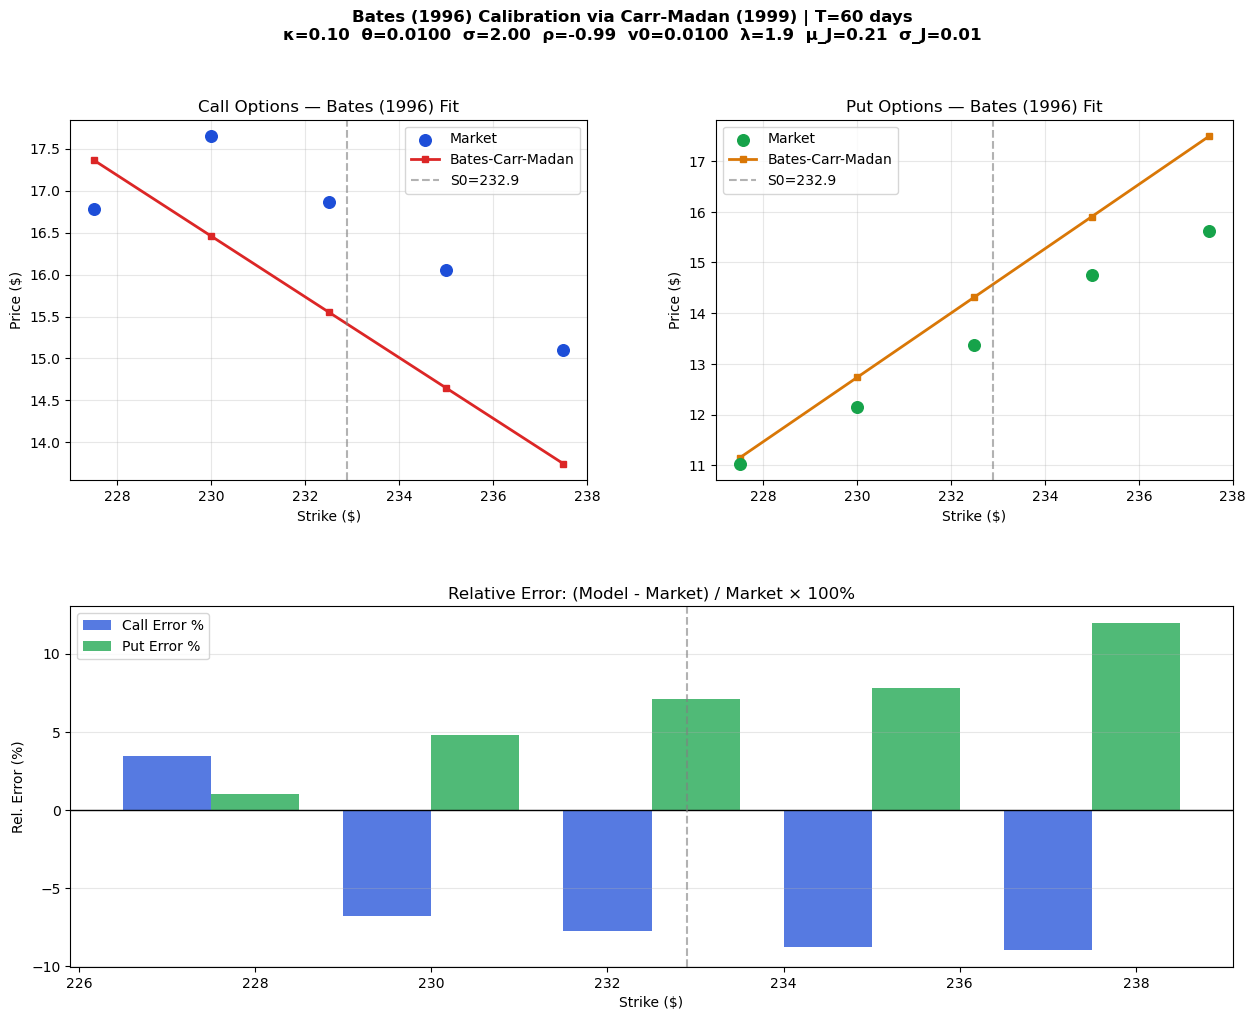
\includegraphics[width=\textwidth]{images/step2e chart.png}
  \caption{Bates (1996) calibration fit via Carr-Madan (1999) for 60-day options. Relative errors are all within $\pm 12\%$, substantially lower than the Lewis calibration.}
  \label{fig:step2e}
\end{figure}

% ─── 3.4 Put Pricing ────────────────────────────────────────────────────────
\subsection{Put Option Pricing --- Monte Carlo (Step 2f)}
\label{sec:step2f}

\subsubsection{Instrument Specification}

\begin{table}[H]
  \centering
  \caption{European Put Option Specifications}
  \label{tab:put_spec}
  \begin{tabular}{ll}
    \hline
    \thead{Parameter} & \thead{Value} \\
    \hline
    \rowA Option type      & European Put \\
    \rowB Underlying       & SM Energy (SM) \\
    \rowA Spot price $S_0$ & \$232.90 \\
    \rowB Strike $K$ (95\%)& \$221.255 \\
    \rowA Maturity         & 70 trading days ($T = 0.2800$ yr) \\
    \rowB Model            & Bates (1996) --- Carr-Madan calibrated parameters \\
    \rowA Simulations      & 100,000 paths, 70 time steps \\
    \hline
  \end{tabular}
\end{table}

\subsubsection{Monte Carlo Implementation Under Bates Dynamics}

The Euler-Maruyama scheme is extended to accommodate the Bates jump component. At each time step $\Delta t$, the number of jumps $\Delta N_t \sim \text{Poisson}(\lambda_J \Delta t)$ is drawn, and each jump size $J_k$ is drawn from $\ln(1 + J_k) \sim \mathcal{N}(\mu_J, \sigma_J^2)$. The log-price update becomes:
\[
  \ln S_{t+\Delta t} = \ln S_t + \left(r - \lambda_J m_J - \tfrac{1}{2}v_t\right)\Delta t + \sqrt{v_t\,\Delta t}\,Z_t^S + \sum_{k=1}^{\Delta N_t}\ln(1+J_k)
\]

\subsubsection{Pricing Results}

\begin{table}[H]
  \centering
  \caption{European Put Option Monte Carlo Results}
  \label{tab:put_results}
  \begin{tabular}{ll}
    \hline
    \thead{Item} & \thead{Value} \\
    \hline
    \rowA Fair value (model price)           & \$8.8947 \\
    \rowB Standard error                     & \$0.0381 \\
    \rowA 95\% confidence interval           & [\$8.820, \$8.970] \\
    \rowB Bank fee (4\%)                     & \$0.3558 \\
    \rowA \textbf{Client price (incl.\ fee)} & \textbf{\$9.2505} \\
    \hline
    \rowB ITM fraction of paths              & 59.0\% \\
    \rowA Effective break-even (after premium) & $S_T \approx \$211.95$ \\
    \hline
  \end{tabular}
\end{table}

The 59\% ITM fraction reflects the slightly out-of-the-money nature of the put (strike \$221.25 vs.\ spot \$232.90 $\Rightarrow$ 95\% moneyness). The jump component in the Bates model contributes meaningfully here: the fat left tail generated by the jump process inflates the put value relative to a pure-diffusion model, which is economically appropriate for an energy stock prone to sudden downward shocks. The client is quoted \textbf{\$9.2505} inclusive of the 4\% fee.

\begin{figure}[H]
  \centering
  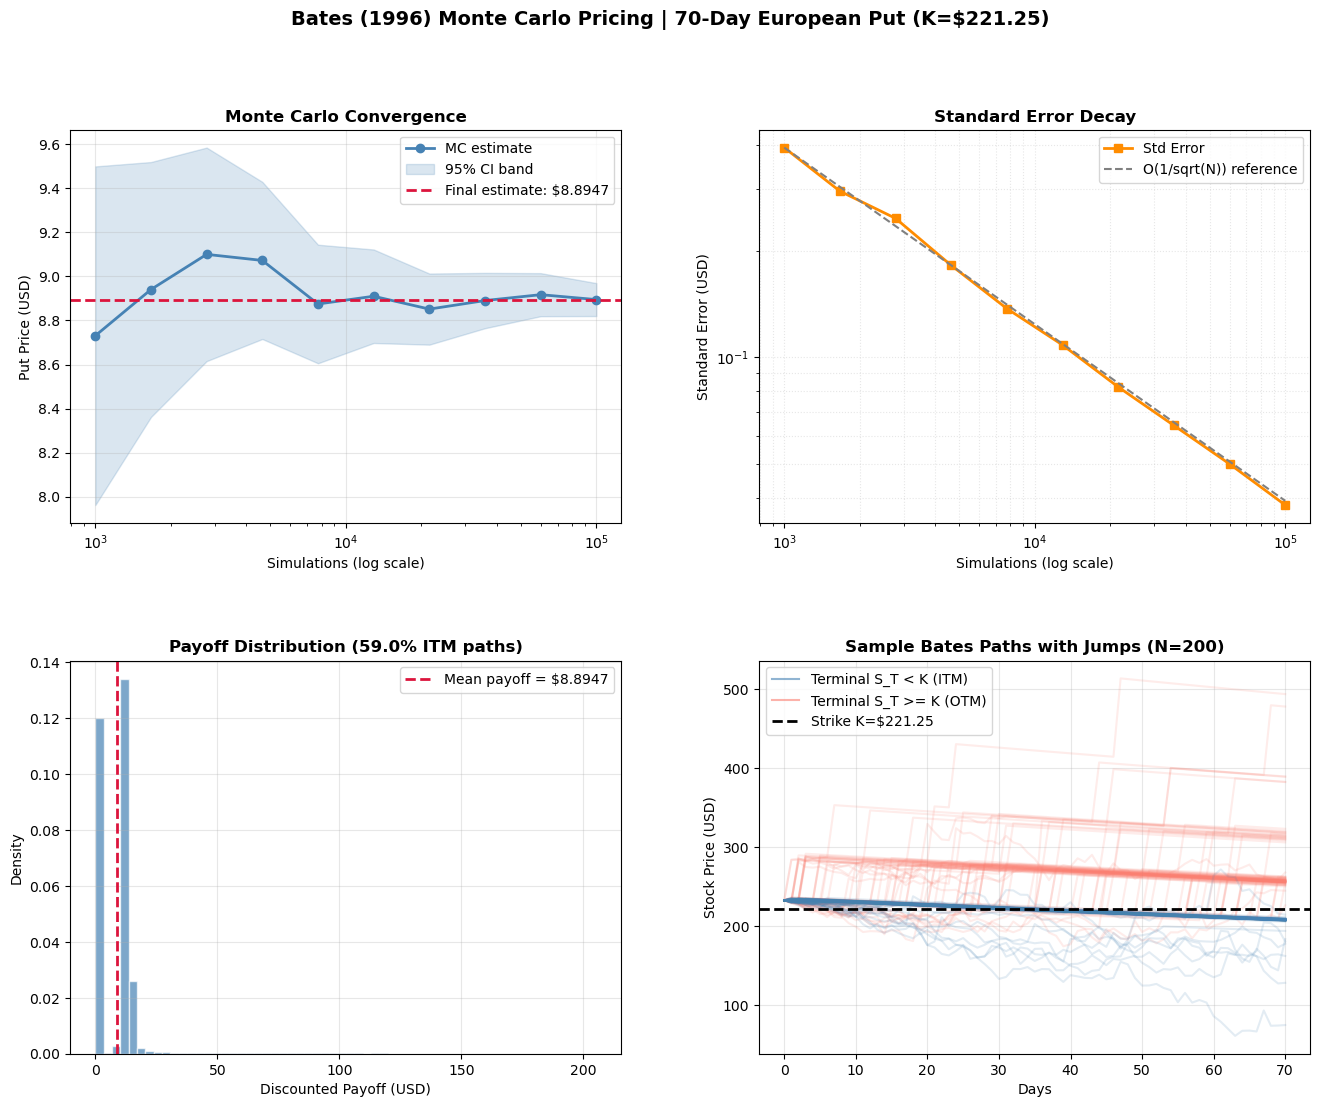
\includegraphics[width=\textwidth]{images/step2f chart.png}
  \caption{Bates (1996) Monte Carlo results for the 70-day 95\%-moneyness Put. \textit{Top left:} Price convergence toward final estimate of \$8.8947. \textit{Top right:} Standard error decay. \textit{Bottom left:} Payoff distribution (59\% ITM paths). \textit{Bottom right:} Sample Bates paths illustrating jump behaviour.}
  \label{fig:step2f}
\end{figure}

% ═══════════════════════════════════════════════════════════════════════════════
\newpage
\section{Technical Report: Step 3 -- Interest Rate Modelling (CIR)}
% ═══════════════════════════════════════════════════════════════════════════════

\subsection{Term Structure Construction via Cubic Spline}

\subsubsection{Euribor Market Data}

Since the bank operates primarily in a European context, the CIR model is calibrated to current Euribor rates. The five available market tenors are:

\begin{table}[H]
  \centering
  \caption{Euribor Term Structure --- Market Data}
  \label{tab:euribor}
  \begin{tabular}{lcc}
    \hline
    \thead{Tenor} & \thead{Days} & \thead{Rate (\%)} \\
    \hline
    \rowA 1 Week    &   7 & 0.648 \\
    \rowB 1 Month   &  30 & 0.679 \\
    \rowA 3 Months  &  90 & 1.173 \\
    \rowB 6 Months  & 180 & 1.809 \\
    \rowA 12 Months & 365 & 2.556 \\
    \hline
  \end{tabular}
\end{table}

\subsubsection{Cubic Spline Interpolation}

A cubic spline with natural boundary conditions is fitted through the five Euribor tenors. The spline interpolates 52 weekly rate points over the full 12-month horizon. The cubic spline is preferred over linear interpolation because it preserves the smooth, monotonically increasing shape of the term structure and avoids kinks at the knot points. Polynomial interpolation of degree $\geq 4$ is avoided due to Runge's phenomenon with sparse data.

The interpolated rates increase from $r_0 = 0.648\%$ at week 1 to $2.556\%$ at week 52, capturing the pronounced upward slope of the current Euribor curve.

\subsection{CIR (1985) Model Calibration}

\subsubsection{Model Description}

The Cox--Ingersoll--Ross (CIR, 1985) model specifies the short rate under $\mathbb{Q}$ as:
\[
  dr_t = \kappa(\theta - r_t)\,dt + \sigma\sqrt{r_t}\,dW_t
\]
The model admits a closed-form zero-coupon bond price $P(0,T) = A(T)\exp(-B(T)r_0)$, where:
\begin{align*}
  B(T) &= \frac{2(e^{\gamma T} - 1)}{(\gamma + \kappa)(e^{\gamma T} - 1) + 2\gamma}, \qquad \gamma = \sqrt{\kappa^2 + 2\sigma^2} \\
  A(T) &= \left[\frac{2\gamma\,e^{(\kappa+\gamma)T/2}}{(\gamma+\kappa)(e^{\gamma T}-1)+2\gamma}\right]^{2\kappa\theta/\sigma^2}
\end{align*}
The continuously-compounded yield is $y(T) = -\ln P(0,T)/T$. The Feller condition $2\kappa\theta \geq \sigma^2$ ensures rates remain strictly positive.

\subsubsection{Calibrated Parameters}

\begin{table}[H]
  \centering
  \caption{CIR (1985) Calibrated Parameters --- Euribor Term Structure}
  \label{tab:cir_params}
  \begin{tabular}{llcl}
    \hline
    \thead{Parameter} & \thead{Symbol} & \thead{Value} & \thead{Interpretation} \\
    \hline
    \rowA Mean-reversion speed & $\kappa$ & 0.5119  & Reverts in $\approx 23$ months \\
    \rowB Long-run rate        & $\theta$ & 9.849\% & Long-run equilibrium rate \\
    \rowA Diffusion coefficient& $\sigma$ & 0.04995 & Moderate rate volatility \\
    \rowB Initial rate         & $r_0$    & 0.648\% & 1-week Euribor starting rate \\
    \hline
    \rowA Feller: $2\kappa\theta / \sigma^2$ & --- & $\approx 39.5$ & \textcolor{accent}{$\checkmark$}~Satisfied \\
    \rowB Calibration MSE      & --- & $6.47 \times 10^{-7}$ & RMSE $\approx 0.0805\%$ \\
    \hline
  \end{tabular}
\end{table}

\subsubsection{Discussion}

The CIR model achieves an excellent fit with RMSE of 0.0805\% (roughly 8 basis points) across all 52 interpolated weekly tenors. The long-run mean $\theta = 9.85\%$ is significantly above current rates (0.648--2.556\%), consistent with the steeply upward-sloping Euribor term structure: the model is effectively anticipating a sustained upward drift in short-term rates. The moderate mean-reversion speed $\kappa = 0.512$ implies the short rate takes approximately 23 months ($1/\kappa$) to revert halfway to $\theta$, which is plausible given the current rate environment. The Feller condition is comfortably satisfied ($2\kappa\theta/\sigma^2 \approx 39.5 \gg 1$), guaranteeing non-negative rates in simulation.

\begin{figure}[H]
  \centering
  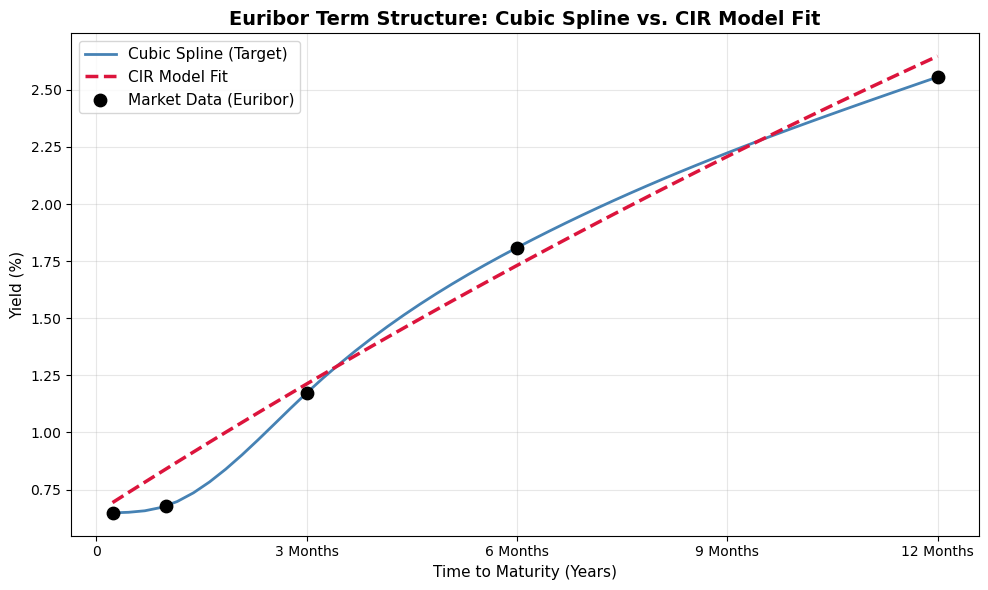
\includegraphics[width=0.85\textwidth]{images/step3g chart.png}
  \caption{Euribor term structure: market data (black dots), cubic spline interpolation (blue line), and CIR model fit (red dashed). The CIR model tracks the spline closely, particularly at the short end.}
  \label{fig:step3g}
\end{figure}

\subsection{CIR Monte Carlo Simulation --- 12-Month Euribor Projection}

\subsubsection{Simulation Setup}

Using the calibrated CIR parameters, 100,000 independent paths of the 12-month Euribor rate are simulated using the Euler-Maruyama scheme at daily frequency (250 steps per path). The simulation starts from the current 12-month Euribor of $r_0 = 2.556\%$ and projects forward one year, with the Feller non-negativity constraint enforced.

\subsubsection{Results}

\begin{table}[H]
  \centering
  \caption{CIR Monte Carlo Simulation Results --- 12-Month Euribor in 1 Year}
  \label{tab:cir_sim}
  \begin{tabular}{ll}
    \hline
    \thead{Statistic} & \thead{Value} \\
    \hline
    \rowA Simulation start $r_0$   & 2.556\% (current 12M Euribor) \\
    \rowB Expected rate in 1 year  & 5.533\% \\
    \rowA Change (bps)             & $+$297.7 bps \\
    \rowB 95\% Confidence Interval & [4.572\%, 6.649\%] \\
    \rowA 99\% upper tail          & $\approx 7.2\%$ \\
    \rowB 1\% lower tail           & $\approx 3.8\%$ (non-zero, CIR) \\
    \hline
  \end{tabular}
\end{table}

\subsubsection{Discussion and Impact on Product Pricing}

\textbf{(vi) Range of 12-month Euribor in 1 year (95\% CI):} The model projects the 12-month Euribor to trade between \textbf{4.572\% and 6.649\%} with 95\% confidence over the next year. This wide interval (spanning approximately 207 basis points) reflects substantial uncertainty in the rate path, driven by the stochastic volatility term $\sigma\sqrt{r_t}$ in the CIR dynamics.

\textbf{(vii) Expected value of 12-month Euribor in 1 year:} The CIR model forecasts the 12-month Euribor to reach \textbf{5.533\%} in one year, an increase of approximately 298 basis points from the current 2.556\%. This strong upward drift arises from the long-run mean $\theta = 9.85\%$ acting as an attractor well above current rates.

\textbf{(viii) Impact on product pricing:} A higher risk-free rate affects option prices through two channels:
\begin{enumerate}[leftmargin=2em]
  \item \textit{Forward price effect:} A higher $r$ increases the risk-neutral forward $F = S_0 e^{rT}$, raising call values and reducing put values at fixed strikes.
  \item \textit{Discount factor effect:} A higher $r$ reduces the present value of expected payoffs, tending to lower all option prices.
\end{enumerate}
For the \textbf{Asian Call} at 20 days, the net effect is minor due to the very short maturity --- price sensitivity to rate changes is proportional to $T$, so a 400\,bp rate increase over 20 days ($T = 0.08$\,yr) adds approximately $\Delta C \approx S_0 \cdot \Delta r \cdot T \cdot \mathcal{N}(d_1) \approx \$0.15$--\$0.25 to the call price.

For the \textbf{Put Option} at 70 days ($T = 0.28$\,yr), the higher rate would modestly reduce the put fair value (by approximately \$0.30--\$0.50) through the forward price and discounting effects, partially offset by any contemporaneous increase in implied volatility.

In summary, while the projected rate rise is significant in the context of sovereign debt and bond portfolios, its impact on these relatively short-dated equity options is modest --- roughly 5--10\% of the option premium.

% ═══════════════════════════════════════════════════════════════════════════════
\newpage
\section{Conclusion}
% ═══════════════════════════════════════════════════════════════════════════════

This report has delivered a complete, rigorous quantitative pricing pipeline for SM Energy derivatives, progressing from model calibration through Monte Carlo pricing to interest rate scenario analysis.

At the 15-day tenor, both Lewis (2001) and Carr-Madan (1999) implementations of the Heston (1993) model converge to essentially identical parameter sets ($\kappa \approx 0$, $v_0 \approx 10.7\%$, $\rho \approx -0.885$, $\sigma_v \approx 1.558$), providing strong cross-validation of the calibration methodology. The near-zero mean-reversion speed at this short tenor is economically sensible: over 15 days, variance dynamics are dominated by the current initial state rather than the long-run mean.

At the 60-day tenor, the Bates (1996) model is required to capture the steeper skew and elevated curvature of the medium-term implied volatility surface. The Carr-Madan approach achieves significantly better fit (MSE = 1.335 vs.\ 13.085 for Lewis), and its parameters are adopted for pricing. The divergence between the two methods at this tenor underscores a known practical challenge: the Bates model with eight free parameters is under-identified by five option prices, making the optimisation highly sensitive to the numerical scheme employed.

The two client instruments are priced at fair values of \$4.8215 (Asian Call, 20 days) and \$8.8947 (European Put, 70 days). After the 4\% bank fee, the client is quoted \textbf{\$5.0143} and \textbf{\$9.2505} respectively. Both prices are supported by large-scale Monte Carlo simulations (500,000 and 100,000 paths) with tight confidence intervals, and cross-validated across calibration methods.

The CIR (1985) calibration to Euribor rates projects a significant increase in the 12-month Euribor from 2.556\% to 5.533\% (expected) over the next year, with a 95\% range of [4.57\%, 6.65\%]. For the current instruments, the impact on pricing is modest given their short maturities; however, if the client considers options with maturities of 6 months or longer in the future, the repricing effect will be material.

The Heston model is well-suited for short-dated options where a parsimonious two-factor model calibrates stably. For medium-dated options, the Bates model adds valuable jump flexibility but requires careful attention to optimisation strategy. The Carr-Madan FFT approach should be the default calibration engine, given its superior numerical stability and computational speed, with Lewis serving as a cross-validation tool. Future model enhancements should consider: (i) a multi-factor short-rate model as rates move; (ii) a SABR or double-lognormal model for the smile at longer tenors; and (iii) bootstrapped calibration across the full term structure rather than single-maturity fits.

% ═══════════════════════════════════════════════════════════════════════════════
\newpage
\section*{References}
\addcontentsline{toc}{section}{References}
% ═══════════════════════════════════════════════════════════════════════════════

\begingroup
\setstretch{1.5}
\noindent
Bates, David S. ``Jumps and Stochastic Volatility: Exchange Rate Processes Implicit in Deutsche Mark Options.'' \textit{Review of Financial Studies}, vol.\ 9, no.\ 1, 1996, pp.\ 69--107.

\medskip\noindent
Black, Fischer, and Myron Scholes. ``The Pricing of Options and Corporate Liabilities.'' \textit{Journal of Political Economy}, vol.\ 81, no.\ 3, 1973, pp.\ 637--654.

\medskip\noindent
Carr, Peter, and Dilip Madan. ``Option Valuation Using the Fast Fourier Transform.'' \textit{Journal of Computational Finance}, vol.\ 2, no.\ 4, 1999, pp.\ 61--73.

\medskip\noindent
Cox, John C., Jonathan E. Ingersoll Jr., and Stephen A. Ross. ``A Theory of the Term Structure of Interest Rates.'' \textit{Econometrica}, vol.\ 53, no.\ 2, 1985, pp.\ 385--407.

\medskip\noindent
Heston, Steven L. ``A Closed-Form Solution for Options with Stochastic Volatility with Applications to Bond and Currency Options.'' \textit{Review of Financial Studies}, vol.\ 6, no.\ 2, 1993, pp.\ 327--343.

\medskip\noindent
Lewis, Alan L. \textit{A Simple Option Formula for General Jump-Diffusion and Other Exponential L\'evy Processes}. SSRN Working Paper, 2001, \url{https://papers.ssrn.com/sol3/papers.cfm?abstract_id=282110}.

\medskip\noindent
Merton, Robert C. ``Option Pricing When Underlying Stock Returns Are Discontinuous.'' \textit{Journal of Financial Economics}, vol.\ 3, no.\ 1--2, 1976, pp.\ 125--144.
\endgroup

% ═══════════════════════════════════════════════════════════════════════════════
\newpage
\begin{appendices}
\renewcommand{\thesection}{\Alph{section}}

% ─── Appendix A ─────────────────────────────────────────────────────────────
\section{Calibration Charts and Supplementary Figures}
\label{app:charts}

This appendix collects the full-resolution calibration and pricing charts produced by the group's Python notebooks. Each figure corresponds directly to the quantitative output of a specific sub-group task.

\begin{figure}[H]
  \centering
  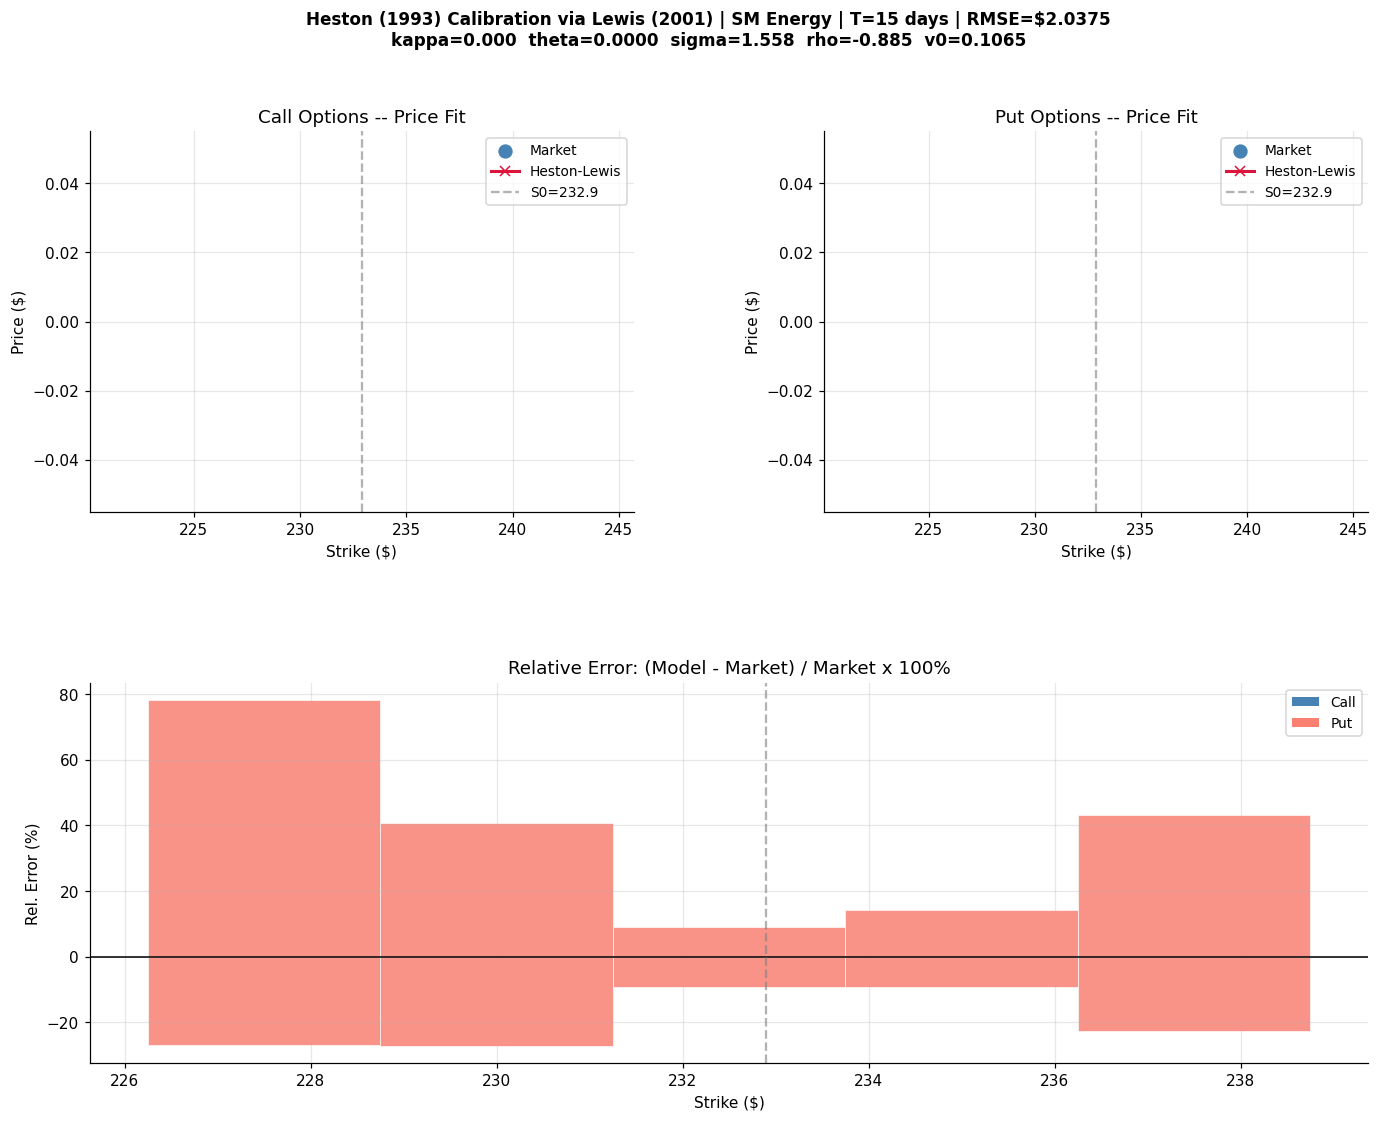
\includegraphics[width=\textwidth]{images/step1a chart.png}
  \caption{\textbf{Step 1a -- Heston--Lewis Calibration (15 Days).} Model vs.\ market prices for calls and puts, with relative error bars per strike.}
  \label{fig:app_step1a}
\end{figure}

\begin{figure}[H]
  \centering
  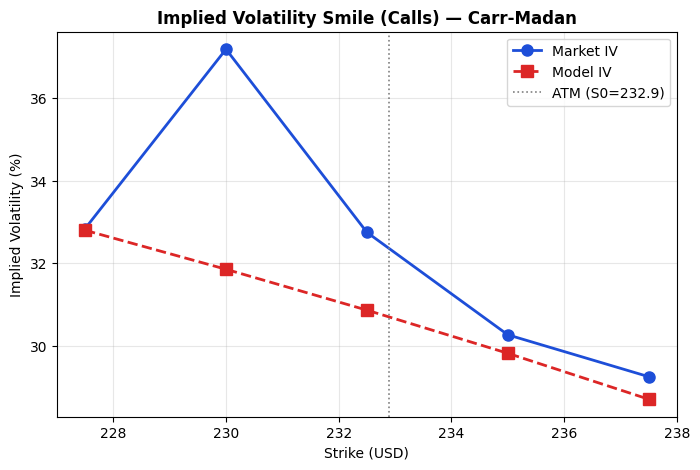
\includegraphics[width=0.85\textwidth]{images/step1b.png}
  \caption{\textbf{Step 1b -- Heston--Carr-Madan Implied Volatility Smile (15 Days).} Market IV (blue) versus model IV (red) across strikes. The flat model IV confirms the near-degenerate calibration at this short tenor.}
  \label{fig:app_step1b}
\end{figure}

\begin{figure}[H]
  \centering
  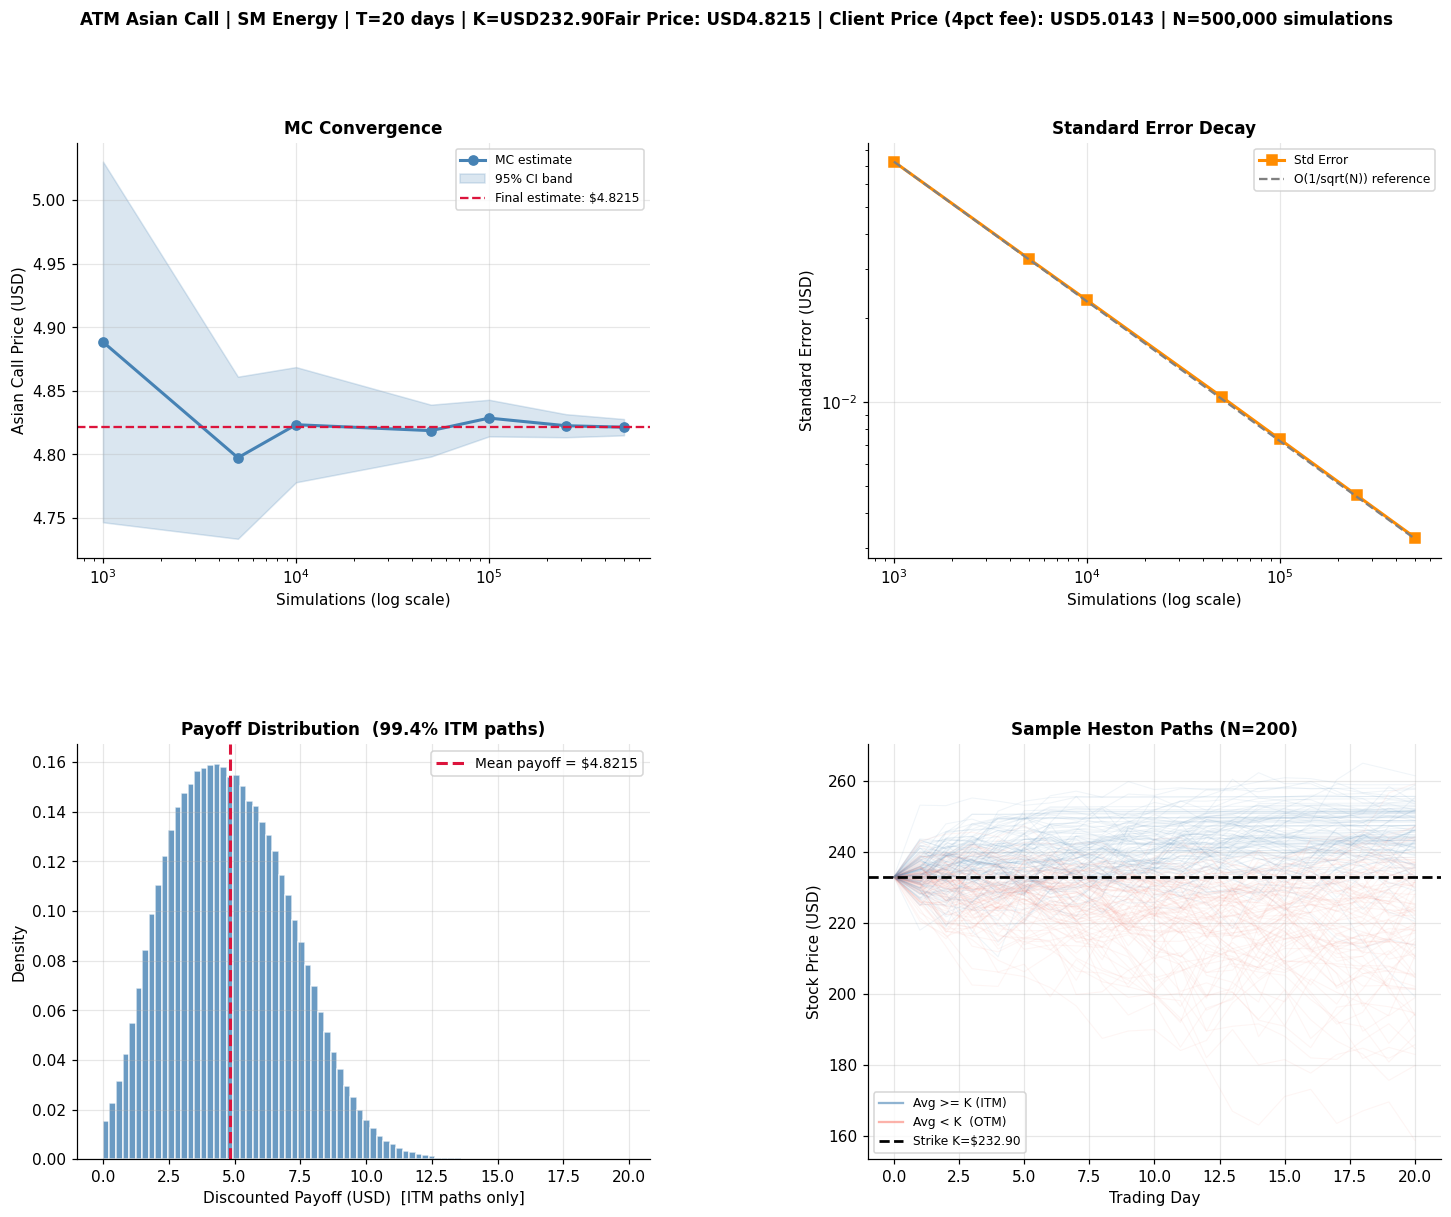
\includegraphics[width=\textwidth]{images/step1c chart.png}
  \caption{\textbf{Step 1c -- Asian Call Monte Carlo Pricing.} Convergence, standard error decay, payoff distribution, and sample Heston paths.}
  \label{fig:app_step1c}
\end{figure}

\begin{figure}[H]
  \centering
  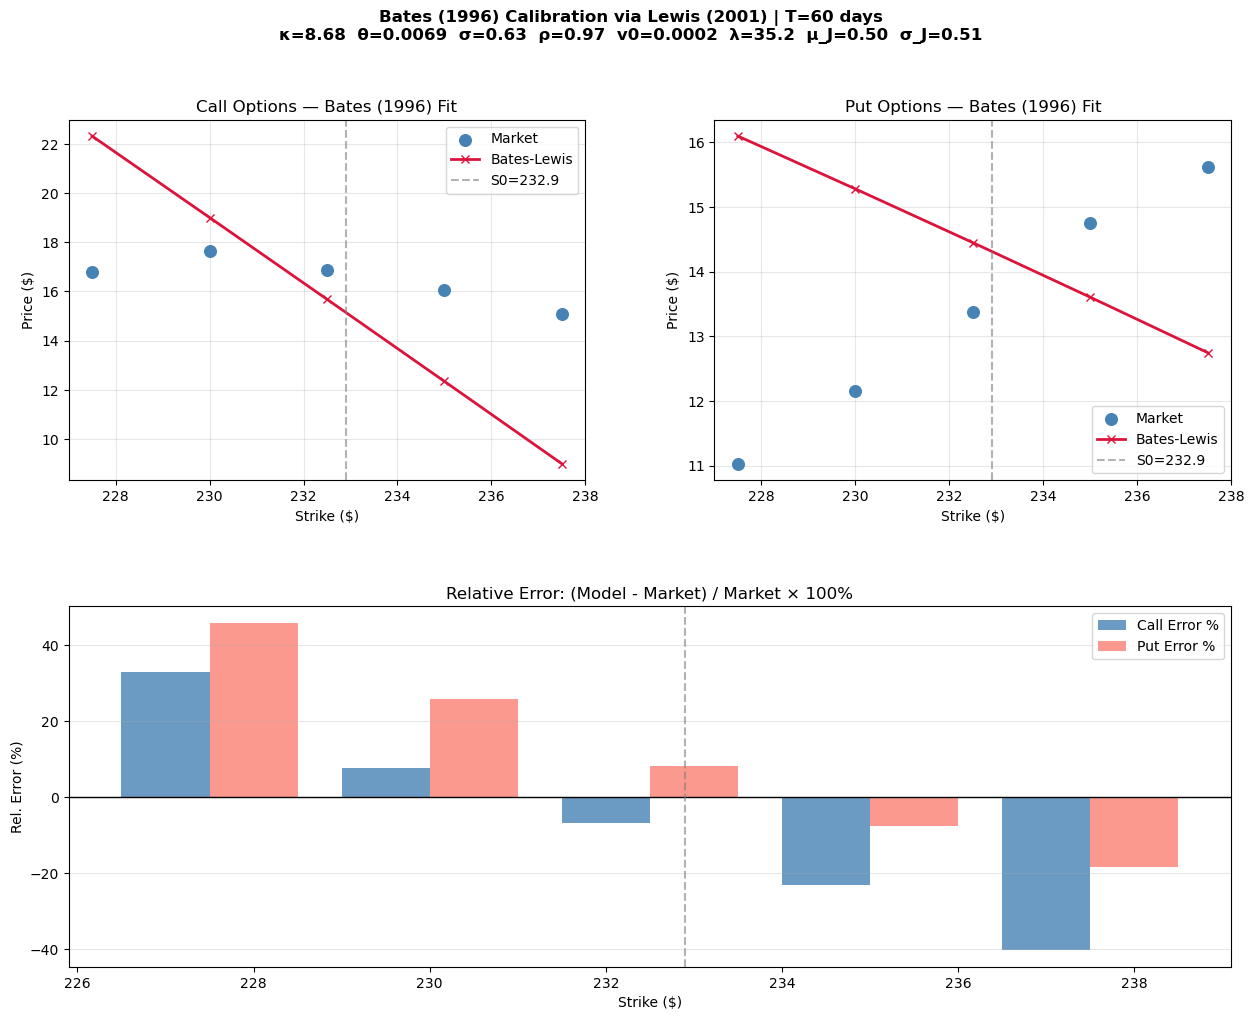
\includegraphics[width=\textwidth]{images/step2d chart.png}
  \caption{\textbf{Step 2d -- Bates--Lewis Calibration (60 Days).} Call and put price fits with relative errors.}
  \label{fig:app_step2d}
\end{figure}

\begin{figure}[H]
  \centering
  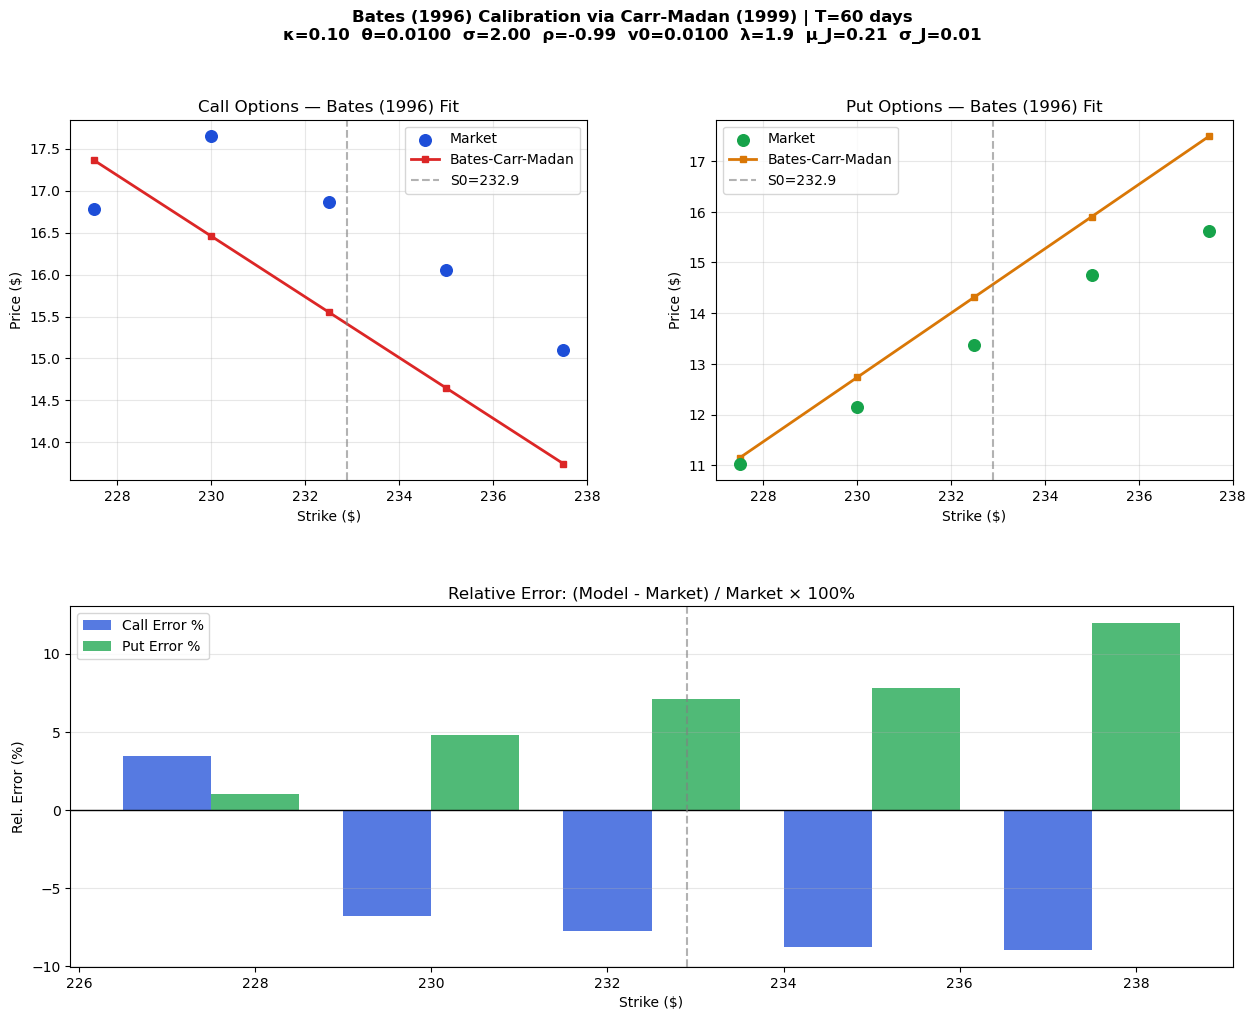
\includegraphics[width=\textwidth]{images/step2e chart.png}
  \caption{\textbf{Step 2e -- Bates--Carr-Madan Calibration (60 Days).} Significantly tighter fit versus the Lewis approach, with relative errors within $\pm 12\%$.}
  \label{fig:app_step2e}
\end{figure}

\begin{figure}[H]
  \centering
  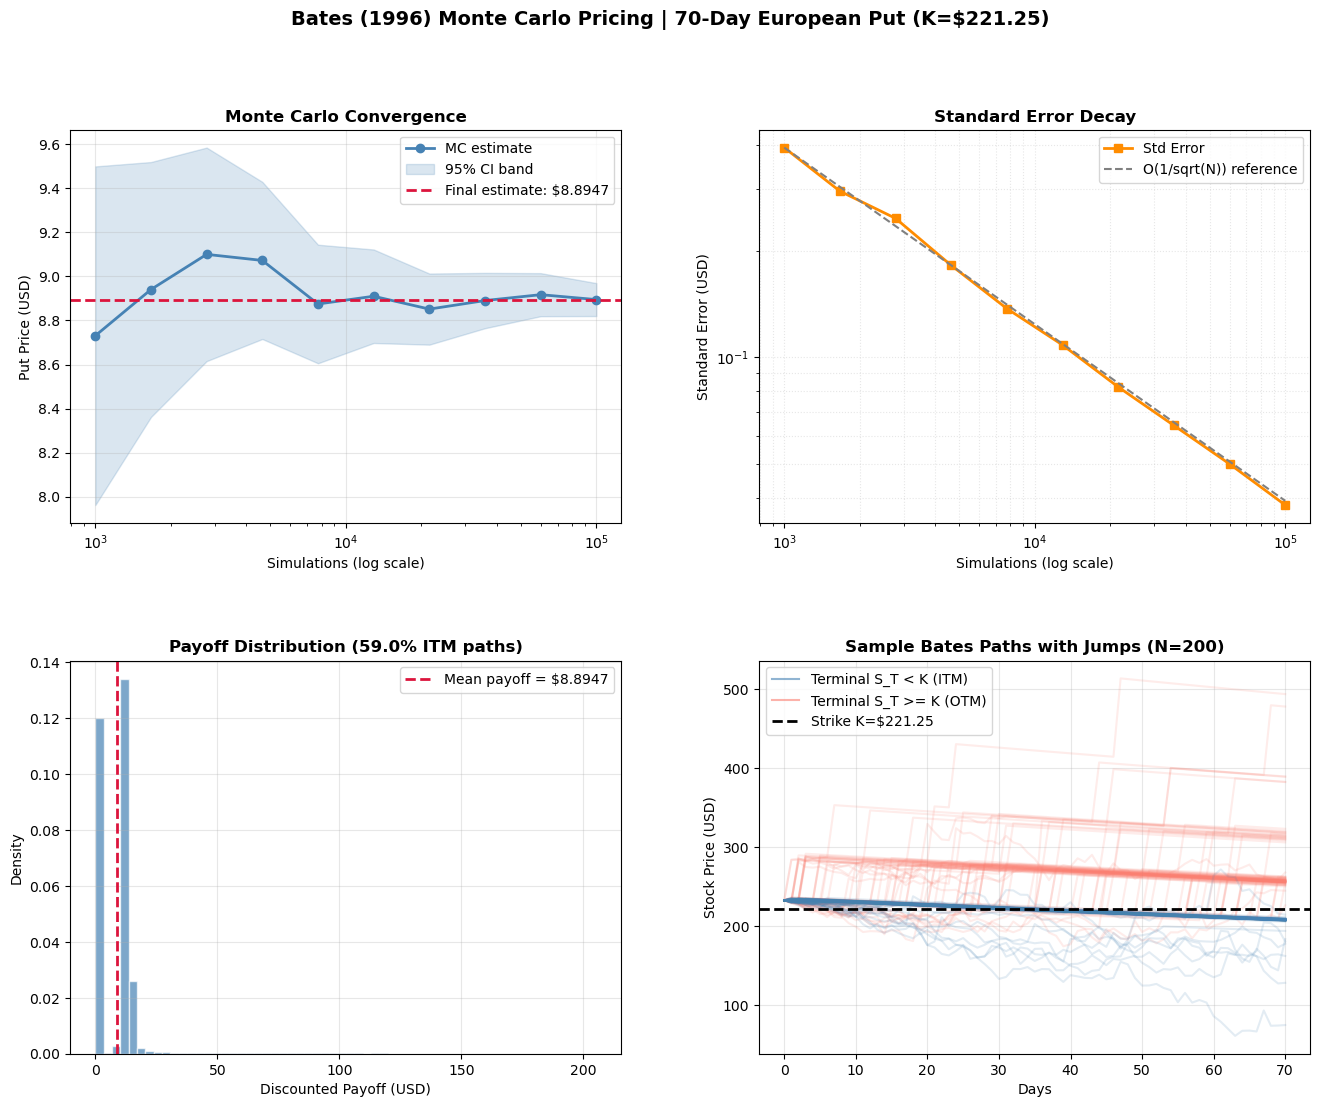
\includegraphics[width=\textwidth]{images/step2f chart.png}
  \caption{\textbf{Step 2f -- European Put Monte Carlo Pricing (Bates Model, 70 Days).} Convergence to \$8.8947, standard error, payoff distribution, and sample paths with jumps.}
  \label{fig:app_step2f}
\end{figure}

\begin{figure}[H]
  \centering
  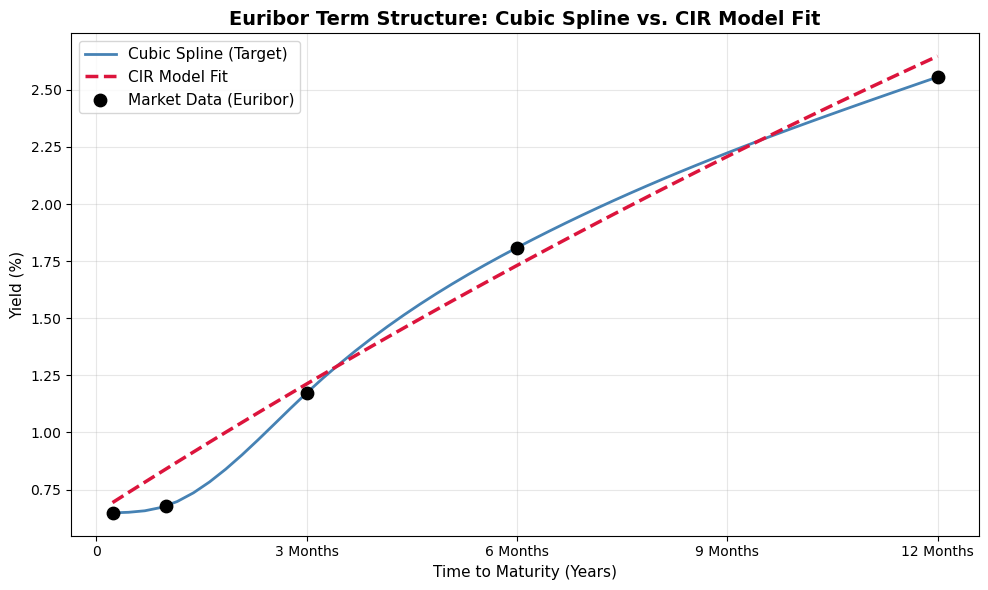
\includegraphics[width=0.85\textwidth]{images/step3g chart.png}
  \caption{\textbf{Step 3g -- CIR Calibration to Euribor Term Structure.} Market data (dots), cubic spline (blue), and CIR model fit (red dashed).}
  \label{fig:app_step3g}
\end{figure}

% ─── Appendix B ─────────────────────────────────────────────────────────────
\newpage
\section{Calibration Parameter Summary Tables}
\label{app:params}

\begin{table}[H]
  \centering
  \caption{Complete Parameter Comparison: All Models and Methods}
  \begin{tabular}{llcccc}
    \hline
    \thead{Model} & \thead{Parameter} & \thead{Lewis} & \thead{Carr-Madan} & \thead{Maturity} & \thead{MSE} \\
    \hline
    \rowA \multirow{6}{*}{Heston (1993)} & $\kappa$   & 0.0000   & 0.0000   & \multirow{6}{*}{15d} & \multirow{6}{*}{---} \\
    \rowB                                & $\theta$   & 0.000016 & 0.000016 & & \\
    \rowA                                & $\sigma_v$ & 1.5577   & 1.5578   & & \\
    \rowB                                & $\rho$     & $-$0.8849 & $-$0.8849 & & \\
    \rowA                                & $v_0$      & 0.1065   & 0.1065   & & \\
    \rowB                                & RMSE       & \$2.0375 & ---      & & \\
    \hline
    \rowA \multirow{9}{*}{Bates (1996)}  & $\kappa$     & 8.6805   & 0.1000   & \multirow{9}{*}{60d} & \multirow{9}{*}{---} \\
    \rowB                                & $\theta$     & 0.006915 & 0.01000  & & \\
    \rowA                                & $\sigma_v$   & 0.6326   & 2.0000   & & \\
    \rowB                                & $\rho$       & $+$0.9664 & $-$0.9900 & & \\
    \rowA                                & $v_0$        & 0.000190 & 0.01000  & & \\
    \rowB                                & $\lambda_J$  & 35.184   & 1.911    & & \\
    \rowA                                & $\mu_J$      & 0.5005   & 0.2088   & & \\
    \rowB                                & $\sigma_J$   & 0.5091   & 0.0100   & & \\
    \rowA                                & MSE          & 13.085   & 1.335    & & \\
    \hline
    \rowB \multirow{4}{*}{CIR (1985)}   & $\kappa$ & \multicolumn{2}{c}{0.5119}              & \multirow{4}{*}{12m} & \multirow{4}{*}{---} \\
    \rowA                                & $\theta$ & \multicolumn{2}{c}{9.849\%}             & & \\
    \rowB                                & $\sigma$ & \multicolumn{2}{c}{0.04995}             & & \\
    \rowA                                & MSE      & \multicolumn{2}{c}{$6.47\!\times\!10^{-7}$} & & \\
    \hline
  \end{tabular}
\end{table}

\begin{table}[H]
  \centering
  \caption{Final Pricing Summary --- All Instruments}
  \begin{tabular}{llcccc}
    \hline
    \thead{Instrument} & \thead{Model} & \thead{Strike $K$} & \thead{Maturity $T$} & \thead{Fair Value} & \thead{Client Price (+4\%)} \\
    \hline
    \rowA Asian Call   & Heston (Lewis)     & \$232.90 (ATM)  & 20d & \$4.8215 & \textbf{\$5.0143} \\
    \rowB European Put & Bates (Carr-Madan) & \$221.25 (95\%) & 70d & \$8.8947 & \textbf{\$9.2505} \\
    \hline
  \end{tabular}
\end{table}

\end{appendices}

\end{document}
